\documentclass[a4paper,12pt]{article}
\usepackage[english]{babel}
\usepackage{setspace,graphicx,epstopdf,amsmath,amsfonts,amssymb,amsthm,versionPO}
\usepackage{marginnote,datetime,enumitem,subfigure,rotating,fancyvrb}
\usepackage[colorlinks=true,linkcolor=blue,anchorcolor=blue,citecolor=blue]{hyperref}
\usepackage[longnamesfirst]{natbib}
\usepackage{ctex}
\usdate
\usepackage{indentfirst}
\usepackage{fusion}
\usepackage{multirow}
\usepackage{fancyhdr}
\includeversion{links}
\iflinks{}{\hypersetup{draft=true}}
\excludeversion{notes}	
\ifnotes{
  \usepackage[margin=1in,paperwidth=10in,right=2.5in]{geometry}%
  \usepackage[textwidth=1.4in,shadow,colorinlistoftodos]{todonotes}%
}{
  \usepackage[margin=1in]{geometry}
  \usepackage[disable]{todonotes}
}
\let\oldmarginpar\marginpar
\makeatletter\let\chapter\@undefined\makeatother
\newcommand{\rhs}[2][]{\smalltodo[color=green!30,#1]{{\bf RS:} #2}}
\newcommand{\rhsnolist}[2][]{\smalltodo[nolist,color=green!30,#1]{{\bf RS:} #2}}
\newcommand{\rhsfn}[2][]{
  \renewcommand{\marginpar}{\marginnote}
  \smalltodo[color=green!30,#1]{{\bf RS:} #2}
  \renewcommand{\marginpar}{\oldmarginpar}}
\newcommand{\textnote}[1]{\ifnotes{{\colorbox{yellow}{{\color{red}#1}}}}{}}
\newcommand{\clearRHS}{\clearpage\thispagestyle{empty}\cleardoublepage\thispagestyle{plain}}
\setcounter{tocdepth}{3}
\newtheorem{theorem}{Theorem}[section]
\newtheorem{assumption}{Assumption}[section]
\newtheorem{proposition}{Proposition}
\newtheorem{conjecture}{Conjecture}
\newtheorem{lemma}{Lemma}[section]
\newtheorem{corollary}{Corollary} \newtheorem{condition}{Condition}
\usepackage{endnotes}
\usepackage{color}
\usepackage{array}
\makeatletter
\def\enoteheading{\section*{\notesname
  \@mkboth{\MakeUppercase{\notesname}}{\MakeUppercase{\notesname}}}
  \mbox{}\par\vskip-2.3\baselineskip\noindent\rule{.5\textwidth}{0.4pt}\par\vskip\baselineskip}
\makeatother
\usepackage{lastpage}
\begin{document}
\selectlanguage{English}
\setlist{noitemsep}
\title{\color{black} FUSION白皮书 \\ [2ex] \begin{large}以区块链为基础的普惠加密金融平台\end{large}
\footnotetext{*FUSION FOUNDATION LTD.是一家注册于新加坡的非营利性组织。E-mail: info@fusion.org。
  }}
\author{FUSION FOUNDATION$^*$}

\date{2017年12月}
\renewcommand{\thefootnote}{\fnsymbol{footnote}}
\singlespacing
\maketitle
\thispagestyle{empty}

\vspace{-.2in}

\renewcommand\abstractname{\large{摘要}}
\begin{abstract}
  \noindent

区块链技术毋庸置疑已经扑面而来。它以一种“信任机器”的方式给人类提供了一种全新高效的协作方法。区块链在金融领域的应用一直受到最大的关注和期待。目前,各种类型的加密数字货币及代币已经基本实现了点对点的价值转移的基本功能,但不可否认,这离现实世界功能完备的金融服务距离还很远,这也正是如今我们看到区块链在金融领域应用雷声大雨点小的根本原因。人类需要一个能够连接各种价值体系、提供完备金融功能、跨接不同社区和代币,以及连接中心化与非中心化组织的价值传输基础设施,以促成价值互联网时代早日来临。

正如互联网时代的到来之时,我们做法并不是去改造“邮政系统”,而是创造了全新“电子邮件系统”。同样,如今价值互联网来临之时,我们希望为其创造全新的系统——一个基于代币的价值转移的基础设施。它能够完成价值在时间与空间上转换,并以分布式的形式,更高效率、更低成本地实现传统金融体系中几乎所有业务,并且实现中心化组织情景下无法想像的功能。它将会把如今相互割裂、各自为阵的加密货币融合在一起,并赋予完备的金融功能。它将引领世界金融进入一个崭新的时代,我们称之为——\textbf{加密金融时代}。

我们为加密金融时代准备了\textbf{FUSION}!FUSION将通过代币私钥的分布式管理在各种区块链代币上面建立一层控制权管理平台,以及通过提供与中心化组织和外部数据源的接口,将各种价值连接起来,从而弥补了现有价值互联网不够互联互通的最大痛点。

FUSION是\textbf{包容的}。它能够融合现今已经存在以及未来产生的加密货币;连接中心化及非中心化组织;容纳身份认证机制和匿名交易机制;引入链上数据和链下数据源等等。FUSION是\textbf{重构性的}。它重新定义了价值转换方式及参与者之间的关系,它将以更加体现金融本质的方法实现价值在时间和空间上的转移,并以一种独特的方式实现金融功能从而使得某些现存的金融产品消失。FUSION是\textbf{高延展性的}。它以虚拟机的形式图灵完备地提供了未来跨越不同代币的加密金融的无限遐想空间,创造各种原先所无法想象的可能性。

本白皮书将在分析价值互联网的基础上提出加密金融的前景,然后提出加密金融时代的FUSION项目的总体设计、关键技术和发展计划。

\end{abstract}

\medskip
\noindent
 \\\\
\medskip
\noindent

\thispagestyle{empty}

\newpage
\thispagestyle{empty}

\noindent
\textbf{\large{使用申明:}}

\onehalfspacing

\onehalfspacing

任何人在未经许可的情况下,出于非商业或教育用途(即收费或商业用途除外),均可使用、复制或分发本白皮书,前提是引用了原始来源和适用的版权声明。

免责声明:本FUSION白皮书仅供参考。 FUSION基金会不保证本白皮书的准确性或达成的结论,本白皮书仅是“按照现在的样子”提供。FUSION基金会不作或明确地否定任何明示或暗示的、法定的或其他方面的陈述或保证,包括但不限于:(1)本白皮书的内容没有错误;(2)这些内容不会侵犯第三方的权利;(3)适用于特定目的、适用性或作用的保证。对于因使用、参考或依赖本白皮书或此处包含的任何内容而引起的任何形式的损害,即使被告知有此类损害的可能性的情况下,FUSION基金会及其关联公司不承担任何责任。在任何情况下,FUSION基金会及其附属公司均不对任何个人或实体因以下事件承担任何形式的责任:损害、损失、责任、成本或费用,无论是直接的还是间接的、后果性的、补偿性的、偶然的、实际的、惩戒性的,或者使用、引用或依赖本白皮书或其包含的任何内容造成的包括但不限于业务、收入、利润、数据、功能、商誉或其他无形损失的任何损失。
\newpage
\thispagestyle{empty}

\renewcommand{\contentsname}{\centerline{目\  录}}
\tableofcontents
\thispagestyle{empty}

\newpage

\clearpage

\onehalfspacing

\setcounter{footnote}{0}
\renewcommand{\thefootnote}{\arabic{footnote}}


\setcounter{page}{1}



\pagestyle{fancy}

\lhead{FUSION:以区块链为基础的普惠加密金融平台}
%\chead{}
%\rhead{}
%\lfoot{}
\cfoot{}
\rfoot{\thepage\ of \pageref{LastPage}}%当前页 of 总页数
%\renewcommand{\headrulewidth}{0.4pt}%改为0pt即可去掉页眉下面的横线
%\renewcommand{\footrulewidth}{0.4pt}%改为0pt即可去掉页脚上面的横线




\section{项目背景与愿景}
\subsection{人类文明发展的核心问题、中心化组织及其问题}

人类既没有尖牙利齿、也不够强壮迅捷。我们的发展依赖于相互合作。人类的合作是建立在分布式市场和中心化的组织基础上的。随着市场的发展和组织的发展,人类文明也不断进步。

建立在以货币为交易媒介的市场上的人类合作,极大的促进了人类发展。但是亚当斯密所说的市场“无形的手”并不是万能的。美国经济学家罗纳德·科斯\citep{coase1937nature}发现,市场也是有成本的。除了交通、信息等成本,市场最大的成本是缺乏信任。由于人脑是黑匣子,任何两个人或任何两个社会组织(包括国家)都存在信息不对称,难免相互猜忌。但是由于作为黑匣子的大脑之间天生缺乏信任的问题,传统的市场经济由于信任产生的成本是很高的。

中心化组织是人们一直解决信任的主要方式。类似观念的人通过国家、政党、企业等组织在一起,促成了近代人类文明的突飞猛进。但是,中心化组织也存在不可克服的问题。首先,组织之间由于缺乏信任机制,加上观念的冲突,造成了残酷的竞争,甚至连年战争和核恐怖。其次,造成资源占有越来越集中在少数人手里,阶层之间的鸿沟越来越明显,这也是法国经济学家托马斯·皮克迪(Thomas Piketty)的新著《21世纪资本论》所论述的问题。最后,中心化组织还存在“单点故障”。大量的资源,包括权力、资本、人才和数据垄断在少数机构手里,一旦被攻破或变节,后果不堪设想。

\subsection{区块链兴起和价值互联网前景}

\subsubsection{区块链的兴起}

分布式的市场是人类文明的阶梯,但存在难以克服的信任问题,为此中心化的方案不断发展,极大地促进了人类的发展,但也成为通向更高级文明的主要障碍。我们如何能够既将分布式市场经济的效率发挥到极致,又减少中心化组织的成本呢? 我们需要以更有效的方式解决信任问题,并发明一种装置将中心化组织与分布式市场更好地协调起来。这是值得我们为之付出的伟大事业。

在这类努力中,以区块链为代表的分布式记账技术可能将对人类解决信任问题起到极为重要的作用。这一技术被《经济学人》的封面文章称为“信任的机器”。可以说,在人类历史上第一次,区块链给人类核心问题,即信任问题的一个彻底的解决途径,即将信任交付给社区和代码,通过各种共识机制建立各种大型分布式账本,以此解决人们合作问题及合作中可能遇到的各种冲突。不仅如此,因为账本是建立在对等网络上的,通过它还可以实现点对点价值转移,还使契约的自动化执行成为可能。这样,陌生人之间不仅能够不经建立信任关系就可以进行交易,而且还能够通过智能合约让交易自动化,从而让人类从走出非洲开始第一次在信任技术上实现飞跃,并开启了创造更高级地人类文明的旅程。

现有大部分技术主要促进了“生产力”的进步,而区块链是对人们的“合作方式”的革新。它正带来一场伟大人类社会组织形态的变革,必将使人类社会形成一种新的社会形态,即建立在区块链基础上的地球村。

\subsubsection{价值互联网前景}

区块链在解决人类核心的信任问题上的巨大的优势,使区块链是一个人类文明升级级别的技术,它的发展在人类为节约交易成本的市场选择冲动下是不可阻挡的。由于每条区块链都可以实现不同于原有信息互联网的信息转发的点对点价值转移,区块链实际上将我们从信息互联网时代带向了价值互联网时代,而这代价值互联网也可以被认为是第二代互联网。

正如信息互联网已经给人类社会带来了重大的社区升级,价值互联网也将带来一场更加完美的社会变革。这是因为,基于区块链技术的价值互联网拥有数字化、智能化、非中心化、包容性等特点。数字化和智能化是信息互联网已经具有的特点,只是现在应用到价值互联网上。非中心化是更本质的特点,它有助于彻底解决人类文明中心化组织带来的发展瓶颈。价值互联网还有更强的包容性:通过私钥控制能够更好保护个人财产,通过共识机制能够更好的解决争议,通过对等网络能够降低交易的进入门槛。

当人们方便地通过互联网发送信息并通过算法对信息编程时,人们迎来了信息互联网时代;当人们方便地通过互联网发送价值并通过智能合约对价值进行编程时,价值互联网的时代也将来临。价值互联网众多优势使它对大部分合作模式具有“高维”优势,各种“价值”都将在区块链上表示,并进行方便的转移和编程。随之而来的,必将是人类合作关系和人类社会的重大变革。

埃森哲的报告\citeyearpar{Accenture}预测区块链经过早期的探索,将在2018年到2024年不断的成长,银行开始见证区块链早期采用者带来的好处,同时监管规则也将逐渐确立,各种新的服务和模式开始出现,原有的流程逐渐被摈弃。2025年后,区块链应用将逐渐成熟,区块链的使用成为主流,同时很好的融合进资本市场体系。世界经济论坛发布白皮书《实现区块链的潜力》\citeyearpar{Worldeconomyforum}大胆预测,到2027年世界GDP的10\%将被存储在区块链网络上。可以预见,正如早期的信息互联网,随着区块链应用的发展,价值互联网也将逐渐成形。

\subsection{价值互联网的瓶颈和现有努力}

\subsubsection{价值互联网的瓶颈}

价值互联网将使人们像管理信息一样管理价值,价值互联网的核心功能是沟通价值。但要实现这一功能,价值互联网要在三个特性上不断进步。首先是互通性。价值存在于不同的区块链、中心化组织和数据中心,价值互联网需要这样的公有链或其它解决方案,它能够沟通不同区块链、不同中心化组织和不同数据源,并且基于基上不仅能够传输价值也能运行智能合约。其次是可扩展性。即价值互联网要能被用在不同的应用场景中,包括金融、工业、政府管理等。最后是可用性。即价值互联网需要有一个丰富的生态并让各种应用顺利地运行起来,让开发人员能够高效率地开放,使用人员能够方便地使用。

图\ref{fig:Characteristics-of-IoV}解释了价值互联网三方面的特性。

\renewcommand\figurename{图}

\begin{figure} [htbp]
\centering 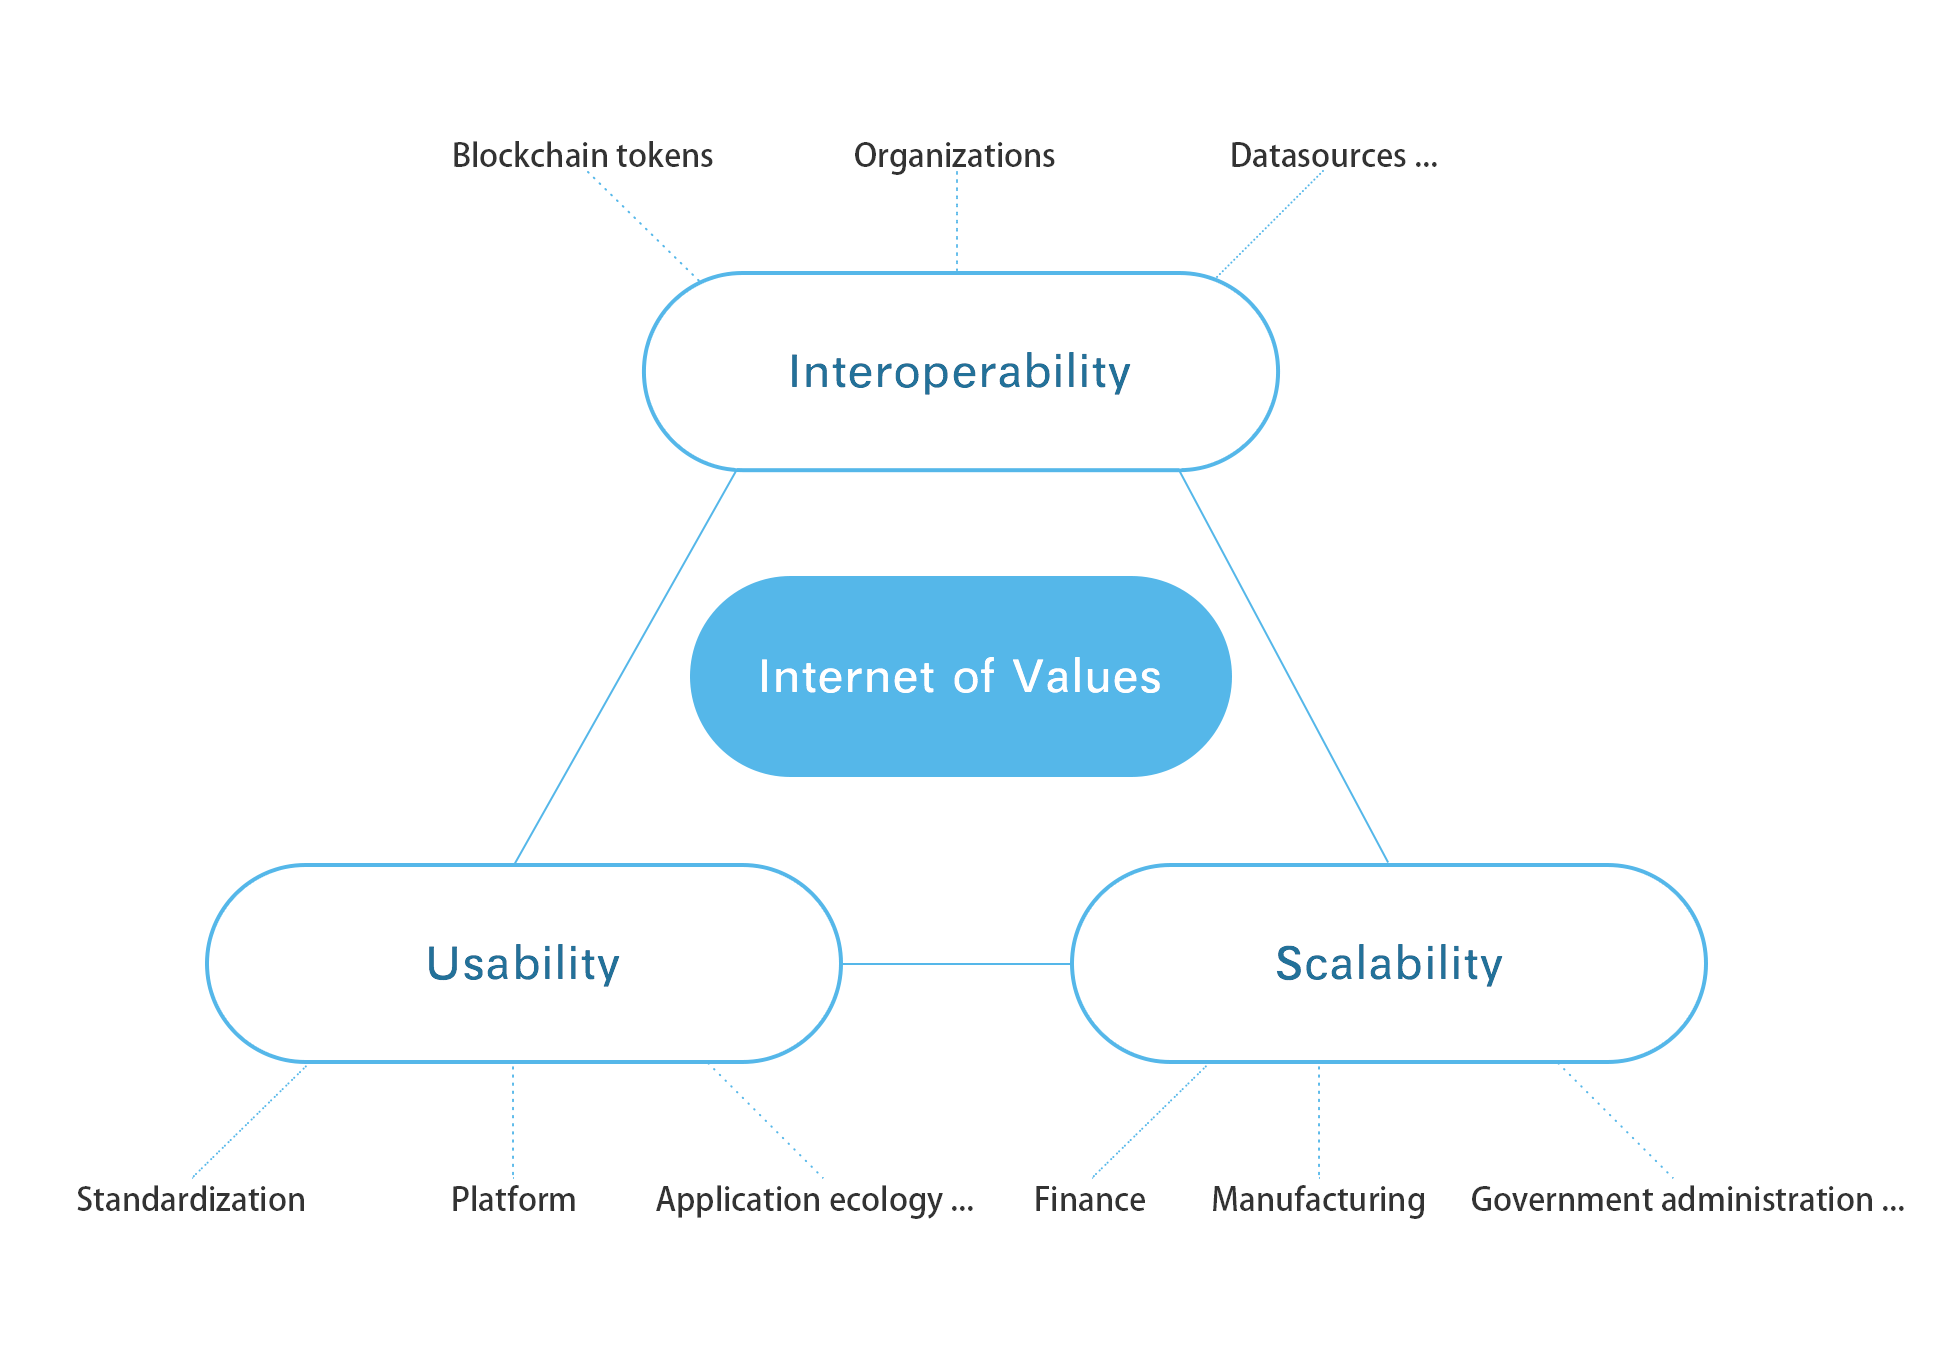
\includegraphics [width = 5in]{pic/Characteristics-of-IoV.png}
\caption{价值互联网性能特征} \label{fig:Characteristics-of-IoV}
\end{figure}


但价值互联网与信息互联网比还处于很初级的阶段,在互通性、可扩展性和可用性三方面都存在瓶颈。

就\textbf{互通性}而言,信息互联网已经可以将文本、图片、音频、视频都统一作为比特信息进行传输和编程,但是,价值互联网上的区块链之间尚且很难通信,更不要说链下资产和链下数据了。

价值互联网不仅需要链间通信,也需要与现有中心化组织的接口及外部数据源的接口。现有的区块链并不能实现与其它区块链的互操作(状态机的同步),使得代币目前仅能通过中心化的方式低效率的进行交易。现在的区块链并不能与现有的中心化组织实现方便的合作,使得链下资产难以实现链上编码。现有的区块链并不能读取链外的数据信息,这使区块链“智能”合约像是一个瞎子,或哑巴,没办法看到,也没办法与外界沟通。

以跨链技术为例,目前跨链通信异常困难,更不要说开发跨链智能合约了。目前已经有数千种代币,但是每一种代币只能在单个区块链上自由转移,并形成了自己的钱包、智能合约开发工具等生态系统。现有的各种各样的区块链生态系统实际上是孤岛生态系统,价值互联网离真正的互联互通还差得很远。

就\textbf{可扩展性}而言,信息互联网已经通过将各种信息编码为比特以及将各种应用场景的沟通逻辑编程为代码,价值互联网得到不断地扩展,但是,价值互联网通过代币化链下价值和将各种场景的交易逻辑映射为智能合约的过程才刚刚展开。

由于互通性有限,价值互联网的可扩展性受到极大的影响。我们很难将现实中的涉及多币种、多组织、多数据源的应用场景映射到链上,形成分布式的解决方案,从而阻碍了链下价值向价值互联网的迁移。

就\textbf{可用性}而言,信息互联网的计算能力、储存能力、带宽等已经能够满足绝大部分信息交换和应用的需求,但是,价值互联网现在要支撑稍重的项目都会显得吃力。价值互联网在标准化、平台化、功能模块化、应用生态化、抗量子攻击等方面都有大量的工作要做。

以上价值互联网与价值互联网的区别可以用下表表示:
\renewcommand\tablename{表}
\begin{table}[!hpb]\small
  \caption{信息互联网与价值互联网}
  \label{tbl:keyproblems}
  \centering
  \begin{tabular}{|c|p{0.35\columnwidth}|l|p{0.1\columnwidth}|}
\hline
特性&信息互联网&价值互联网 \\
\hline
互通性&文本、图片、音视频可混合编程& 代币、资产、身份、数据等难以混合编程\\  
可扩展性&Web、APPs、ERP、IoT等纷纷上线& 仅有少数落地项目\\  
可用性&标准化、操作系统、编程、分布运算、人工智能等完善的生态& 标准化、编程语言、应用框架等初级阶段\\  
\hline
 \end{tabular}
\end{table}

三种瓶颈中,互通性最为迫切,它需要实现不同代币的价值转移和智能合约;可扩展性的迫切性其次,而可用性的迫切性最末。可用性是一个综合性、长期性的基础工作,但互通性和可扩展性已经极大地阻碍了价值互联网的发展,可能有短期解决方案,已经成为目前最迫切需要解决的两大瓶颈。

\subsubsection{现有努力}

现在一些区块链项目正在尝试在这三方面努力。

在互通性方面,跨链点对点转账有一些不重要的尝试,而跨链智能合约的分布式解决方案还没有出现。现有的跨链通信技术最主要的是侧链技术,但主链与侧链在通信延时、安全、并发等方面的问题都不容易解决。更有甚者,很多方案里主链与侧链的接口依然是中心化的解决方案。跨链智能合约方面的努力在中短期是难以成功的,因为目前单链共识机制的标准化进程还远没有成熟,更不要说多链之间达成共识了。

为了实现代币之间的交易,这样简单的互通,现有的解决方案仍然是各种各样的代币交易所。目前中心化交易所爆炸式的发展直接证明了可行的跨链通信的分布式解决方案还没有出现。

在可扩展性方面,大量链下价值和交易场景要实现上链还很不容易。目前,公有链上通过类似ERC2.0协议进行的ICO项目正不断增加,但现实世界的大量资产,包括金融资产、固定资产、实物资产、各种衍生品等都很难可靠的映射到线上。链下大量的交易场景,只要涉及重的运算、链下机构频繁的操作和对外数据的需求的,都较难映射到链上。人们进行着相关的努力,但由于缺乏跨链的通信机制,使这一进程严重受阻。

在可用性方面,分布式计算、高吞吐时储存和通信,可编程、互操作、模块重用方面都还比较初级。目前有提出的很多方案,比如通过搭建私有链来解决问题,或者指定固定节点完成记账共识等。但长远看,要真正实现价值互联网的愿景,可用性的提高还是需要完全公有链和分布式的方案。这需要在硬件性能、算法、共识机制、密码学等多方面不断的努力。

总之,互通性、可扩展性和可用性是目前价值互联网的主要瓶颈,但该行业还没有出现很好的解决方案。

\subsection{加密金融蓝图}

\subsubsection{价值互联网与加密金融}

价值互联网的本质是将各种链下价值映射到链上,从而实现链下的价值能够被智能合约处理。价值互联网使人与人合作非中心化、去中介、普惠、可编程等成为可能。这些显然的优点将让各种有价值的东西争相上链。随着区块链瓶颈的不断攻克,必然造成价值互联网不断快速成长。

价值上链的过程要求将价值从业务逻辑中抽象出来。可见,价值互联网上天生具有很强的金融属性。价值互联网上金融属性特点强的应用,我们可以称其为价值互联网上的金融应用。我们把价值互联网上进行的金融活动称为\textbf{加密金融(cryptofinance)}。之所以,冠以“加密”二字,是因为这种通过代币化形成的证券化金融资产是通过加密技术进行控制,这与传统的金融资产已经有了巨大的区别。

由于价值互联网是基于信息互联网的,所以价值互联网包含了信息互联网的大部分特性。但是,就信息传输而言,两者有一点显著的不同,价值互联网是建立在对等网络和UDP协议之下的,这正是价值互联网出现诸多瓶颈的原因。未来的价值互联网的性能将逐渐逼近现有的信息互联网,从而使业务场景及其金融交易都可以无缝地在同一程序中实现编程。但是就目前情况看,我们预计这还需要比较长的时间,目前的价值互联网将主要承载金融应用,即加密金融应用将是目前价值互联网的主要应用。

\subsubsection{加密金融资产的特点}

在讨论加密金融蓝图之前,我们有必要说明一下“加密金融资产”,即价值互联网中的“价值”。我们已经看到了信息互联网对于我们生活的深刻影响,我们也可以同样预想价值互联网将给我们的生活带来巨大的变革,甚至有过之而无不及。我们也很明白信息互联网上信息的类型,但很少有人讨论价值互联网上的“价值”的特点。

首先,价值互联网上的价值是区块链代币,价值映射到价值互联网的过程就是资产代币化(tokenization)的过程。如果链上记账符号能够代表链下资产的产权、收益和控制权等,那么链下资产就实现了链上的表示,并且成为价值互联网的一部分。价值互联网正是通过这一过程让越来越多的价值进入,并通过分布式帐本防止“双花”,从而可以使价值不需要中介就可以像转移像发送信息一样方便,对价值进行编程也像对信息进行编程一样地简单,从而让我们看到了像以前信息互联网的对应的价值互联网的前景。这一规律已经在以太坊ERC2.0协议下初见端倪,但以太坊上实现代币化的资产还不够广泛,也没法实现跨链和跨数据源的交互,其可用性也存在问题。

其次,代币化的过程就是价值资产证券化的过程,实现链下价值转化为链上加密金融资产。由于代币可以无限细分,在时间和空间上转移,可以用于抵押、借贷、保险等金融业务。所以,各类价值上链的过程就是实现资产证券化并变成通过私钥就可以控制的加密金融资产的过程。

最后,可代币化的价值将更加的多样化。只要上链有利可图,在价值互联网上身份、签名权、数据、投票权等都可能被映射到价值互联网上。所以,价值互联网上的价值可能比传统金融市场中的资产更加广泛。我们认为未来的价值互联网容纳现有市场中交易的大部分价值。显然,现有大量的有价值的物品,比如土地、房物、艺术品、才智等大量有价值的东西也还没有很好的实现链上的表示。但随着各种“价值上链技术”不断发展,资产代币化将发展成一个崭新的行业,越来越多的价值将得以上链流通。

\subsubsection{加密金融的现状}

存在于价值互联网上的金融活动才刚刚起步。虽然,有人认为加密货币已经开始往生活的方方面面渗透,并且增速很快,但其总价值只有几千亿美元,与现有全球金融的规模比,可算是九牛一毛。要知道,全球土地及房产市场、股票市场、大宗商品市场、外汇市场、债券市场、衍生品市场等的价值都是数十万亿、上百万亿甚至上千万亿的市值。

除了规模外,加密金融在功能上,除了转帐和ICO外,其它基本是空白。表\ref{tbl:cryptofinance}比较了传统金融与加密金融在各方面的情况。

\renewcommand\tablename{表}
\begin{table}[!hpb]\small
  \caption{传统金融与加密金融}
  \label{tbl:cryptofinance}
  \centering
  \begin{tabular}{|c|p{0.35\columnwidth}|l|p{0.1\columnwidth}|}
\hline
功能	&	传统金融	&	加密金融	\\
\hline
货币与支付	&	法币,SWIFT,银行间支付系统,信用卡,移动支付	&	代币,钱包	\\
权益	&	天使, VC, PE, IPO, 股票交易所	&	ICO,ECR20,交易所	\\
负债	&	贷款,国债,债券	&	几乎没有	\\
保险	&	人寿保险,财产保险,再保险	&	几乎没有	\\
衍生品	&	远期,期货,期权,互换,ABS,CDS	&	几乎没有	\\
另类投资	&	土地,房产,艺术品,大宗商品,对冲基金	&	几乎没有	\\
财富管理	&	信托,基金,私人顾问	&	几乎没有	\\
\hline
 \end{tabular}
\end{table}

除了规模和金融功能外,从总的说来,加密金融有三方面的不足:

一是市场。加密金融市场在深度、广度和生态的完善上都严重不足。

二是互通性。现在的加密金融难以做到跨链交易、跨组织交易、跨数据源交易。

三是可编程性。现在智能合约不够自动化、智能化和功能不完备。自动化方面,现在智能合约必须要通过外部发起一笔交易才能执行;智能化方面,现有触发机制不能通过外部事件触发;在功能方面,只能对代币做整体转移,不能将所有权和使用权分开编程。

图\ref{fig:Characteristics-of-Cryptofinance}图示了加密金融在以上三方面的不足。

\begin{figure} [htbp]
\centering \includegraphics [width = 5in]{pic_cn/Characteristics-of-Cryptofinance.png}
\caption{加密金融的不足} \label{fig:Characteristics-of-Cryptofinance}
\end{figure}

\subsubsection{加密金融蓝图}

通过以上分析我们可以提出结论,各种价值上链的过程,实际上是某种价值的证券化为加密金融资产的过程,并且同时实现了去中介、数字化和可编程。实际上,资产代币化活动和代币在价值互联网上所进行的金融活动都属于加密金融的范畴。加密金融将帮助价值进入价值互联网,并成为价值互联网的主要组成部分。

加密金融最主要的特点是,金融产品主要是在区块链上表示的,其产权主要是由私钥控制的,金融活动主要是在区块链上通过特殊的智能合约完成的。由于加密金融的先进性,它将对现有的金融形成“超维”打击,链下的资产将代币化为加密金融资产,而链上金融产品将主要是由代币的智能合约表示。由于智能合约主要影响不同加密金融资产的地址上的“金额”,所以智能合约可以相互嵌套,表达各种复杂的金融逻辑,形成一些传统金融中没有可能实现的金融应用。

加密金融活动主要包括两个层面的内容,一是价值代币化为加密金融资产。这可能需要各种服务业,包括会计师事务所、律师事务所、托管机构、国家法律体系等才能实现,这可以称为“加密金融外围服务”;第二个层面是加密金融资产在链上进行的金融活动。这主要通过去中心化的区块链上的智能合约完成的,这可以称为“加密金融应用”。它们共同构成了加密金融活动。

特别指出的是,区块链不能解决一切问题,中心化组织是人类制度进化的重要产物,将在未来与区块链化社区长期共存,并一起促进价值互联网的形成。所不同的是,中心化组织将成为加密金融外围服务业的主要服务主体;而区块链将成为加密金融市场的基础设施。所以,加密金融将把现有的人们都纳入到金融活动中。可以预见,随着加密金融的发展传统金融机构将逐渐转型为加密金融的外围服务和金融应用的服务机构。

加密金融还有一个必须强调的特点,即加密金融是普惠的,所以我们也可以称加密金融为\textbf{普惠加密金融}(inclusive cryptofinance)。这一判断源于加密金融所构建的基础即价值互联网是普惠的。价值互联网门槛低、自由进入、容易退出、产权完全由个人支配、能容纳各种各样的价值,所以作为价值互联网一部分的加密金融也是普惠的。加密金融不排斥一切可以上链的价值,不排斥所有愿意参与的人或中心化组织,他们都将成为价值互联网生态的一部分。

加密金融让我们看到现有金融体系升级的美好前景,但建立在价值互联网上的加密金融也受到价值互联网瓶颈的影响。虽然大量的加密金融应用可以从现有业务场景中抽象出来,对价值互联网的可用性要求并不高,但是要创造加密金融的蓝图,我们首先要解决现有互通性和可扩展性的问题。特别是,我们要解决“区块链孤岛”的问题,在此基础上我们才能实现丰富的加密金融生态系统。

\subsection{FUSION愿景}

针对加密金融的美好前景和现有价值互联网的瓶颈,我们提出了FUSION项目。FUSION的愿景(参见图\ref{fig:FUSION's-interoperability})是要建立加密金融时代的平台级公有链,它能够连接各种价值、提供完备金融功能、跨接不同社区和代币,以及连接中心化与非中心化组织的关键价值传输基础设施,以促成价值互联网时代早日来临。


\begin {figure} [htbp]
\centering 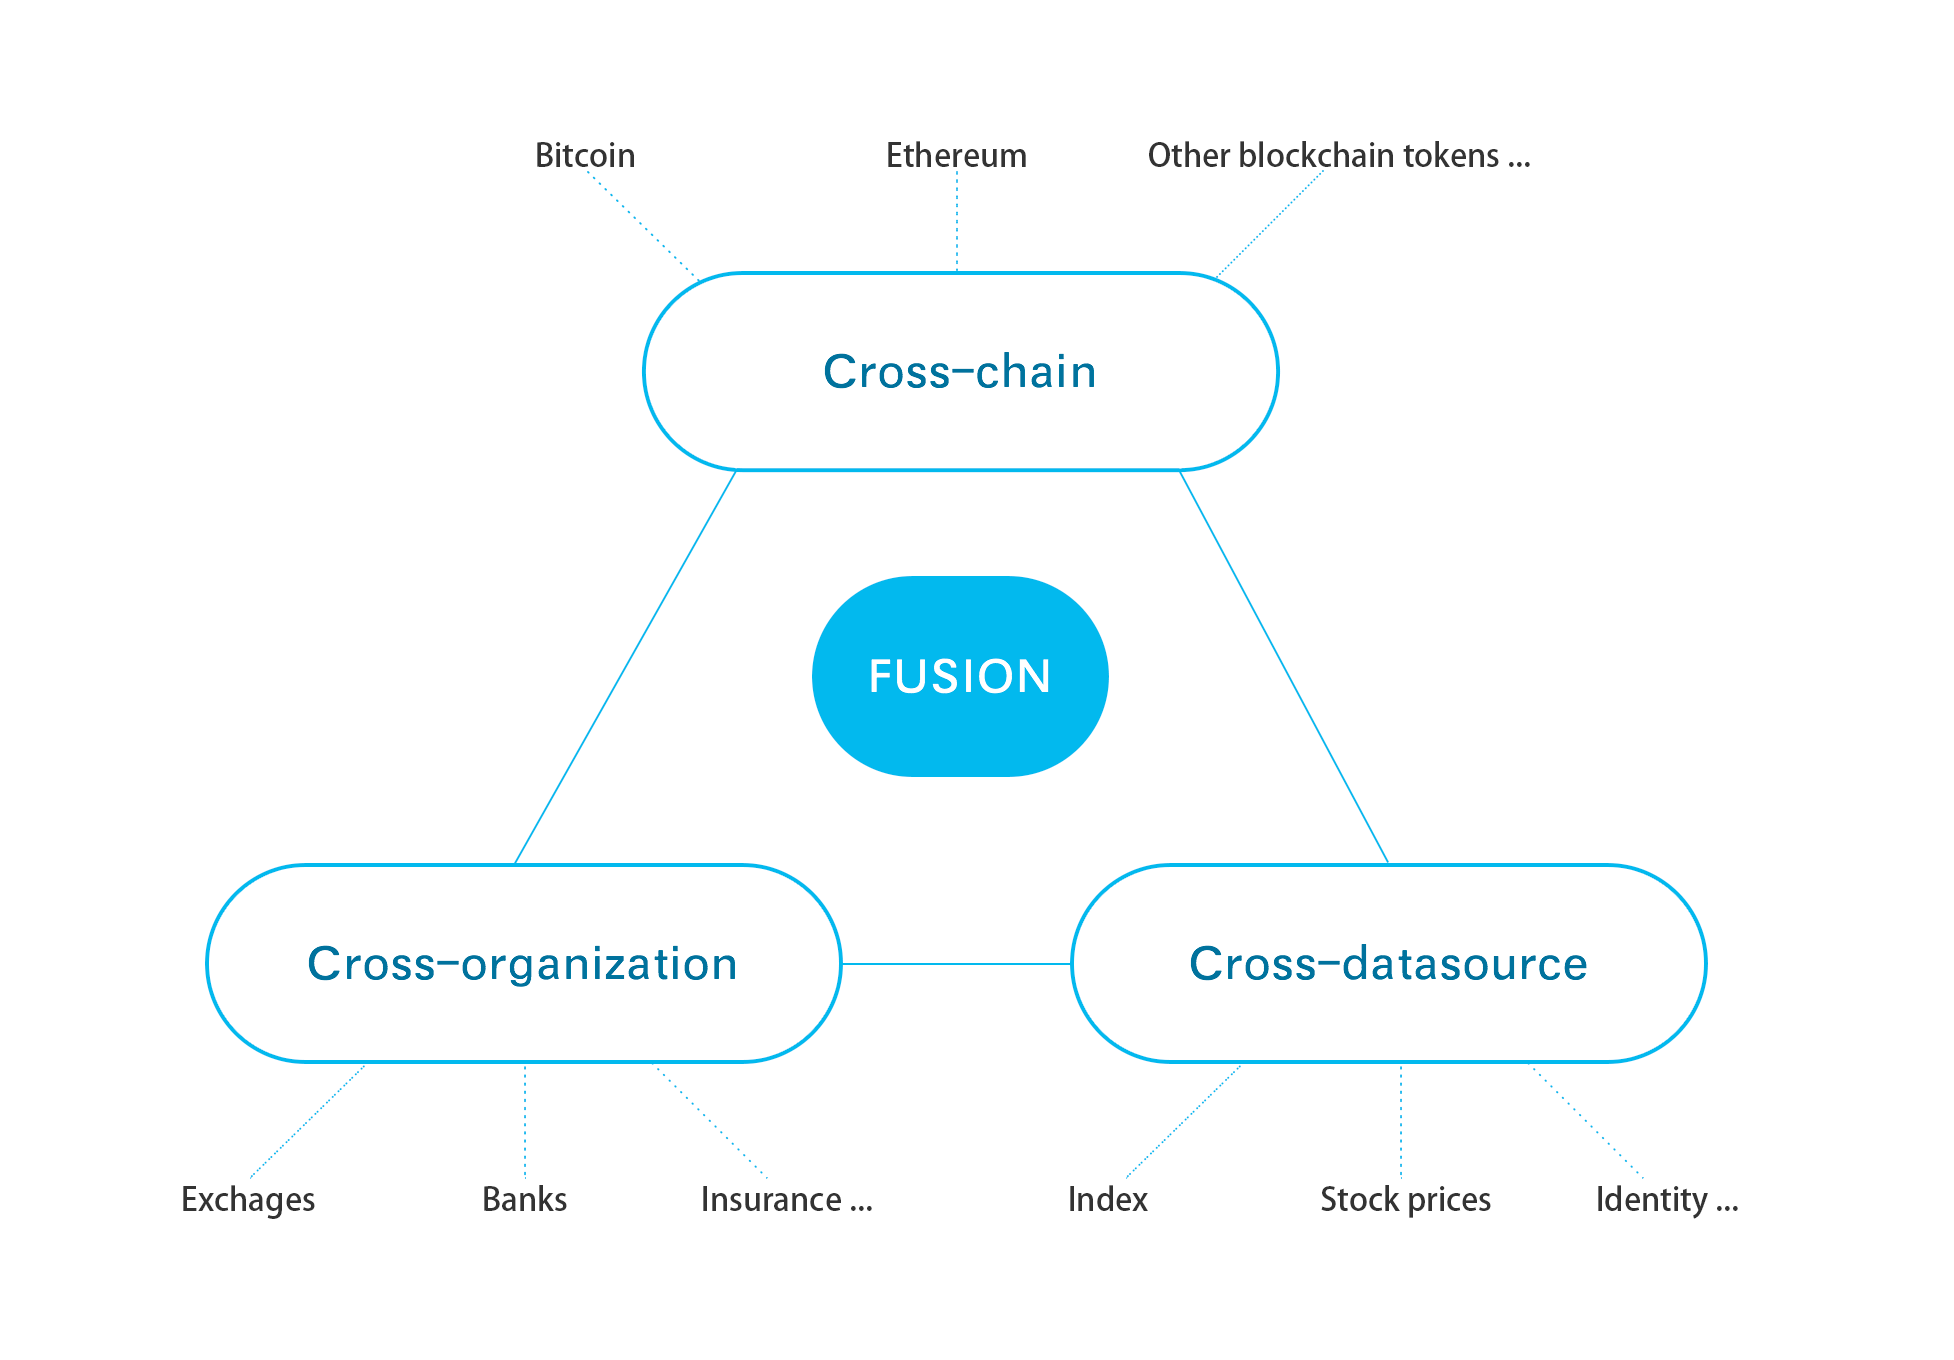
\includegraphics [width = 5in] {pic_cn/FUSION's-interoperability.png}
\caption {FUSION的愿景} \label {fig: FUSION's-interoperability}
\end {figure}


\section{FUSION设计和架构}
\subsection{设计思路}

\subsubsection{分布式节点私钥控制}

由上述可知,区块链的兴起使人们看到了价值互联网的前景,而价值互联网代表着人类文明的未来。但是,价值互联网在互通性、可扩展性和可用性还存在瓶颈,这使得现有价值互联网很难实现跨链的价值转移、跨链智能合约和重的应用,也阻碍了大量价值迁移到其上。但是,能够突破这些瓶颈的方案还没有产生。由于可用性是一个长期逐渐完善的过程,互通性和可扩展性就成为目前主要应该解决的问题。

由于加密金融资产是以代币形式呈现,只要能够实现多币种智能合约就能够极大的提高价值互联网的互通性,也让可扩展性的提高变得极其容易。现在的跨链技术一般是侧链技术通过双向锚定,在侧链交易,并通过多重签名实现退出。这样的做法,只能实现原子性的转账,各方面的性能都不高。

我们需要建一条公有链,并以一种更加创新的方式让不同币种都能映射到这条公有链上,从而可以使这些代币在同一条链上实现多币种智能合约,极大的提高价值互联网的互通性,并成为加密金融的基础设施。它不仅可以沟通不同区块链上的价值,还应该能够提供与中心化组织和链下数据源的接口,以提高区块链的可扩展性。

如何能够实现不同币种映射到一条新的公有链呢?\textbf{我们设想通过一条公有链以分布式的方式安全地控制各种区块链上的代币私钥,从而建立一个分布式的管理代币控制权的区块链。它就像价值互联网上的“高速公路”,能够轻松实现各种代币之间的价值转移及面向加密金融服务的多币种智能合约。}

由于各种价值,包括区块链代币、链下资产、身份数据和其它各种数据,都是“价值”,通过各种代币化技术就可以实现价值的链上表示。未来各种应用场景将产生各种各样的区块链。但是,由于区块链代币都是由私钥控制的,只要能够实现将代币私钥控制权转交给一条公有链的分布式节点管理,就可以实现价值互联网的价值的通过该公有链的智能合约进行分布式管理。通过图灵完备的智能合约,该区块链还可以以更加精妙的形式提供加密金融的各种功能。

这条连接一切代币的区块链不需要完成各种具体应用场景的复杂逻辑,它的目的是在所有区块链上建立一层管理层,从而实现所有代币的交互。由于它不需要跑过重的应用逻辑,现有的可用性已经能够使它承载加密金融的各种功能。它能够极大程度地解决价值互联网互通性和可扩展性方面的痛点并成为加密金融重要的基础设施。

这条公有链,作为基础设施,处于经济世界最底层,虽然肉眼看不到,但却能够强力地不仅将各种价值融合起来,让价值互联网更加完整,还将释放出惊人的价值。这就像核聚变的力量,不仅将各种粒子强力地融合在一起,让世界更完整,还释放出惊人的能量。所以,我们称这条公有链为FUSION。

FUSION是一个加密金融平台级的应用项目。另外,由于FUSION平台拥有价值互联网的分布式、低门槛、包容、民主、去中介等特点,能够跨链、跨组织和跨数据源,所以FUSION加密金融平台也是一种普惠金融平台。

\subsubsection{要解决的关键问题}

由以上分析我们知道,FUSION项目要解决的问题是:FUSION将建立一条公有链,通过分布式节点控制各种代币的私钥,从而将各种代币映射到FUSION上,并实现跨链的智能合约功能。它还将提供接口以沟通链下组织和数据源,以此极大地改善目前价值互联网的互通性和可扩展性,并使自己成为服务于价值互联网的普惠加密金融平台。

要解决这一问题,就需要解决以下几个分问题:

首先,互通性。通过将各种区块链代币的私钥置于分布式节点的控制之下,从而将这些代币映射到同一公链之上,使得所有的代币在同一条链上具有互通性。

第二,可扩展性。为链下资产和数据提供代币化的接口,并通过链下中心化组织管理这些资产和数据,从让智能合约能够实现与现实世界的价值和数据的通信。

最后,可用性。要承载大量的代币就需要充分利用分布式节点进行分布式并行计算,以提高FUSION的性能。

实际上,要实现我们的愿景解决的问题还有很多,而FUSION项目也将随着这些问题的解决不断进化。以下是我们概括出来的需要解决的一些问题。其中一些问题,我们已经基本解决,但需要完善,另一些问题,正在着手解决。具体见表\ref{tbl:keyquestions}。

\renewcommand\tablename{表}
\begin{table}[!hbp]
  \caption{关键问题列表}
  \label{tbl:keyquestions}
  \centering
  \begin{tabular}{|c|l|l|}
\hline
编号	&	类型	&	名称	\\
\hline
1	&	经济模型	&	FUSION经济模型\\
2	&	密钥控制	&	跨链通迅接口	\\
3	&	 	&	FUSION代币账户体系	\\
4	&	 	&	FUSION的节点多重签名并防止受到攻击	\\
5	&	 	&	FUSION平台的密钥对节点不可见	\\
6	&	FUSION共识机制	&	工作量证明与权益证明机制设计	\\
7	&	 	&	签名奖励	\\
8	&	 	&	处罚机制	\\
9	&	 	&	节点分工问题	\\
10	&	 	&	抵押机制	\\
11	&	跨币种智能合约	&	金融契约通用模型	\\
12	&	 	&	多币种智能合约的功能	\\
13	&	 	&	虚拟机机制	\\
14	&	 	&	交易撮合机制	\\
15	&	 	&	支付应用	\\
16	&	 	&	主要应用场景	\\
17	&	跨组织接口	&	与银行的接口方式	\\
18	&	 	&	与交易所的接口方式	\\
19	&	 	&	与中心化组织接口的标准化	\\
20	&	跨数据源接口	&	链下数据接口设计	\\
21	&	FUSION生态系统	&	高校社区建设办法	\\
22	&	 	&	技术设计建设办法	\\
  \hline
 \end{tabular}
\end{table}


\subsection{设计目标}

FUSION的目标是以区块链技术构建加密金融应用运行的基础平台,在这个平台上多种代币可以通过智能合约自由交互,实现价值互通。因此,FUSION的设计需要考虑加密金融应用在系统功能,以及系统在安全性、可靠性、效率等方面的特性要求,以及未来发展相匹配的处理能力。具体而言,包括下列技术需求:

(1)系统功能
\begin{itemize}[itemindent=1em]
	\item 具有多代币交互的功能。
	\item 能够实现代币、金融功能和触发条件之间关系的表达,实现加密金融应用场景和内容的编程。
	\item 具有通过输入多种类型的触发条件,完成金融契约或交易的功能。
\end{itemize}

(2)系统特性
\begin{itemize}[itemindent=1em]
	\item 代币资产的安全性。
	\item 系统的鲁棒性。
	\item 对应用响应和处理的效率。
	\item 实现在加密金融应用的开发过程中屏蔽底层区块链技术,简化加密金融的应用开发。
\end{itemize}

(3)规模化
\begin{itemize}[itemindent=1em]
	\item 能够满足大规模加密金融应用的需求。
	\item 能够在系统达到大规模的情况下保持合理的能效比。
	\item 能够平稳地保持区块大小和区块链数据存储规模在一个合理的范围内。
	\item 能够在系统自身规模和应用规模扩张的情况下,保持对节点计算能力的要求在一个合理的范围内。
\end{itemize}

\subsection{体系架构}

针对上述在系统功能、特性和规模化上提出的技术需求,FUSION的设计思路是实现分布式控制权管理,构建面向加密金融的智能合约和实现分层混合共识机制这三个主要方向。由此构成FUSION的体系架构如下图所示。

\begin{figure}[htbp]
	\centering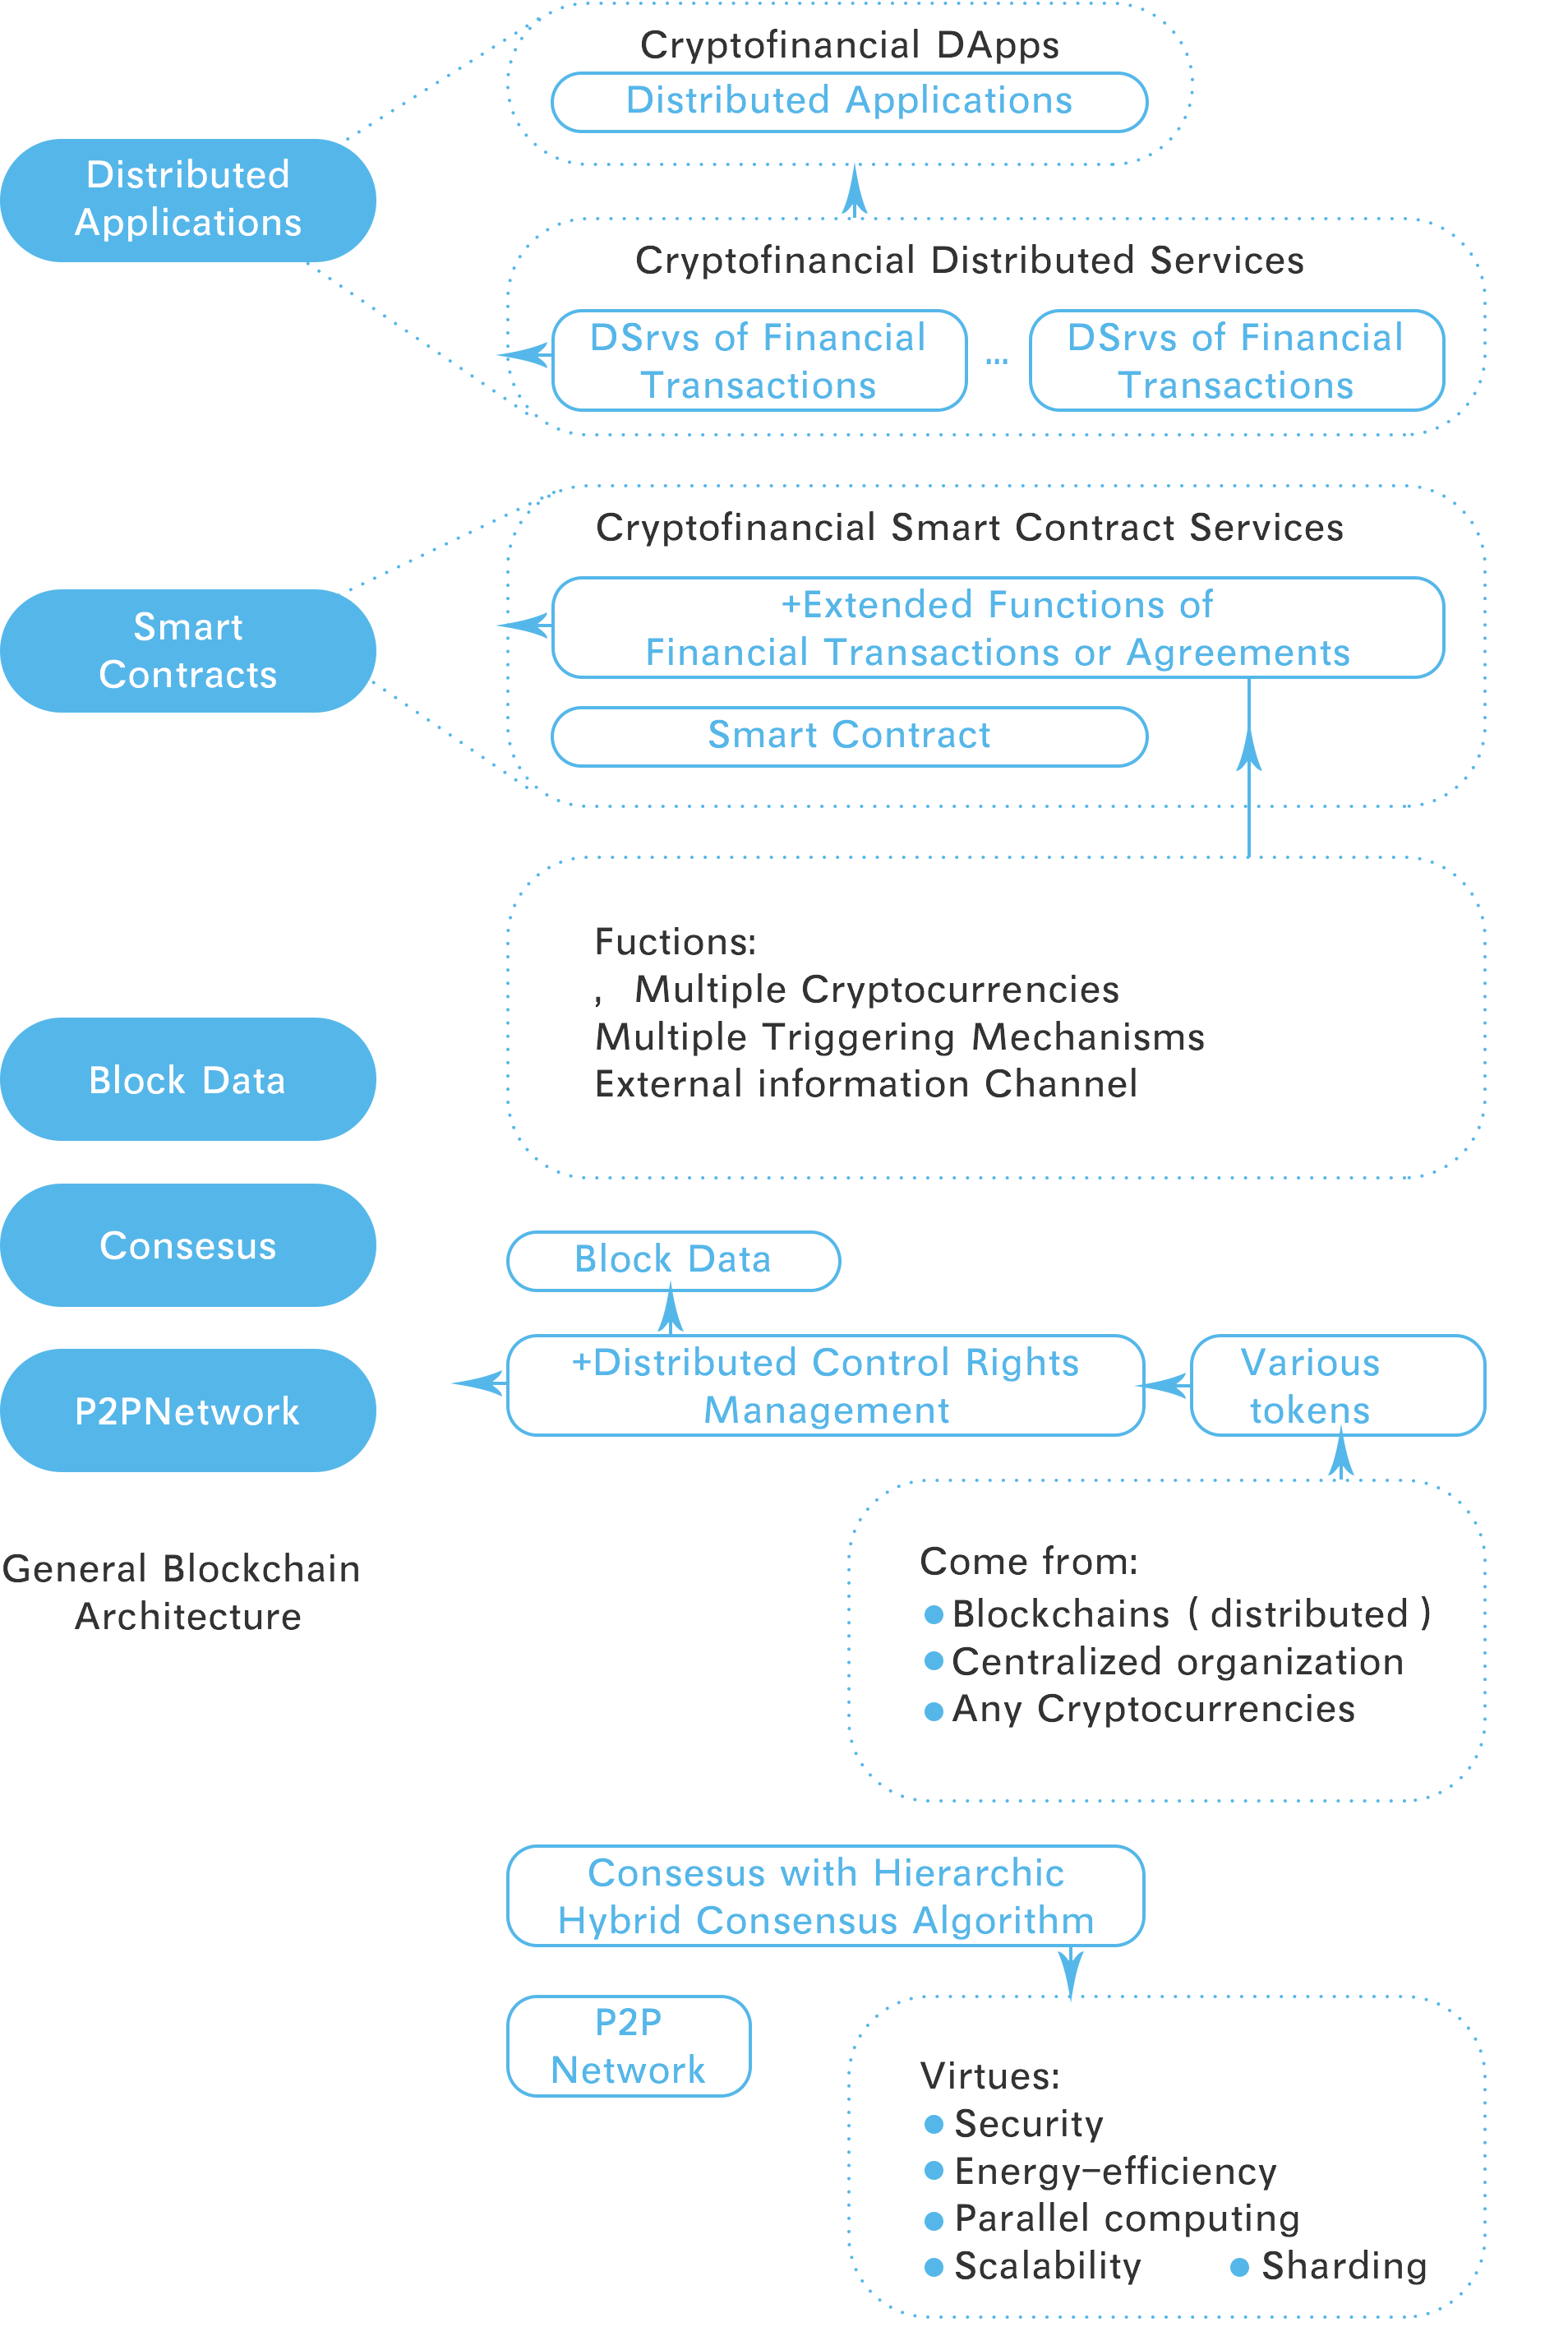
\includegraphics[width=\linewidth]{pic/Architecture.png}
	\caption{FUSION架构}\label{fig:Architecture}
\end{figure}

接下来,按照自下而上的顺序,通过比对现有一般的区块链体系架构,对FUSION的设计规划进行进一步说明。

(1)以分层混合共识机制作为FUSION系统共识层的具体实现。
\begin{itemize}[itemindent=1em]
	\item 分层混合共识机制通过实现区块生成节点的随机性,保障记账节点的不可预测性,增强FUSION系统的安全和鲁棒性。
	\item 分层混合共识机制通过实现PoW和PoS的平衡,结合两者的优点,避免算力或权益的集中化趋势,实现FUSION系统合理稳定的能效比。
	\item 分层混合共识机制通过内建的分组并行机制,实现对于交易的并行处理。
	\item 分层混合共识机制通过应用分层计算,实现应用数据的分片处理和存储,降低对于记账节点在计算能力和存储能力上的要求。
	\item 分层混合共识机制在节点和算力与当前系统规模和应用规模之间进行动态调整,实现系统对大规模应用的扩展能力。
\end{itemize}

(2)增加“分布式控制权管理”层。
\begin{itemize}[itemindent=1em]
	\item 通过分布式控制权管理,数字资产在参与加密金融的过程中,以分布式的密钥生成和保管方式替代现有中心化的私钥生成和保管的方式,提升数字资产的安全性。
	\item 通过分布式控制权管理,实现将不同代币化资产映射到一条链环境上,实现不同代币化资产之间的自由交互。
	\item 通过映射,使多种代币化资产成为加密金融应用操作的对象,赋予这些代币原来不具备的跨时间、跨空间和跨对象的加密金融属性。
\end{itemize}

(3)对现有的智能合约实现金融扩展功能,从而构建面向加密金融的智能合约。
\begin{itemize}[itemindent=1em]
	\item 增加智能合约对两种及两种以上的代币化资产的关系定义能力。
	\item 增加多种智能合约触发条件,满足加密金融应用交易和契约实现过程中对不同形式触发条件的要求。
	\item 定义链外数据通道,支持对接不同的数据源,将链外数据引入FUSION作为加密金融应用所需的数据。
\end{itemize}

(4)构建分布式的加密金融基础服务,增加“加密金融分布式服务(Distributed service, DSrv)”层。
\begin{itemize}[itemindent=1em]
	\item 封装加密金融的共性基础应用成为DSrv,为上层加密金融DApp的开发屏蔽底层区块链技术,从而简化加密金融DApp的开发促进加密金融DApp的丰富。
\end{itemize}

(5)实现“加密金融DApp”层。
\begin{itemize}[itemindent=1em]
	\item 实现面向加密金融DApp的开发、部署和运行。
\end{itemize}

接下来,将对FUSION在分布式控制权管理,面向加密金融的智能合约和分层混合共识机制的设计和实现加以进一步阐述。

\section{分布式控制权管理}
\subsection{资产映射和分布式控制权管理}
{\bfseries{分布式控制权管理(Distributed Control Rights Management,DCRM)}}将个人或组织手中的数字资产控制权移交为由非中心化的区块链管理的过程。密钥以分布式产生和分布式存储的方式,保障了没有任何一个个体能够接触到完整的私钥,也就意味着不存在一个单点能够获得处在分布式控制权管理状态下数字资产的控制权。

我们称在FUSION上生成与被管理对象的相应的数字化资产记账符号的过程为{\bfseries{加密资产映射(cryptoasset mapping)}}。代币通过映射可以与其他被映射资产之间自由交互。

实现和解除分布式控制权管理的操作称为Lock-in和Lock-out。

\textbf{Lock-in(Cryptoasset Lock-in)}是对所有以密钥管理的数字资产,实现分布式控制权管理和资产映射的过程。

\textbf{Lock-out(Cryptoasset Lock-out)}是Lock-in的逆向操作,包括两部分:解除分布式控制权管理和解除资产映射。完成Lock-out后数字资产的控制权交还给所有者,恢复为密钥整体存储和中心化的管理方式。

对数字资产采用分布式控制权管理,增加了现有数字资产的安全性,流动性和加密金融应用功能,从而进一步提升了数字资产的价值。

\subsection{提高数字资产的安全性}
加密资产的控制权体现为私钥控制权。以比特币\citep{Satoshi2008}举例,私钥的本质是一个随机数,比特币的私钥算法为对随机数运行SHA256哈希算法生成256位随机数。在前面加上版本号,后面添加压缩标志和附加校验码(经过2次SHA-256运算,取两次哈希结果的前四字节),然后再对其进行Base58编码,就可以得到WIF(Wallet import Format)格式的私钥。公钥由私钥经过secp256k1椭圆曲线算法生成,比特币地址由公钥经过哈希函数(RPIEMD+SHA)生成。

目前,不管数字资产在个人或交易所手里,其密钥都完整的存储于一个中心化单点。这个单点可能是用户自己,也可能是提供钱包的第三方或者是中心化的交易所等等。因此,密钥的泄露、被盗取以及第三方恶意侵占都会造成用户数字资产的巨大损失,而以上种种情况已经都在数字资产领域发生。

分布式控制权管理从两个方法来获得数字资产的安全性:

(1) 密钥分片

将完整的密钥分成若干个部分的过程称为密钥分片,其中的每一个部分称为该密钥的一个分片。分片后的密钥从生成到保存、使用都不需要进行重组,从而使得在任何地方和任何时候都不会出现完整的私钥。

(2) 分布式保管

将分片后的密钥交给非中心化系统中的不同节点分别保管称为分布式保管。分布式保管的过程中,每个节点只会接触到密钥中的一个或几个分片,任何节点靠这几个分片都不足以重组出密钥,从而最大程度地降低密钥泄露的风险。

分布式保管中密钥交由非中心化系统的保管方式,可以彻底避免发生被第三方恶意侵占的行为。

\subsection{实现多币种之间的金融功能}

\subsubsection{实现不同数字资产间的交互}

通过智能合约可以实现数字资产间更丰富的应用。但是,现在的智能合约只能在同一条链上处理同一类数字资产。当前对于数字资产跨链交易的研究,主要集中在两种不同数字资产之间原子交易的实现。它的局限性在于只实现两个对手之间的交换这一种操作,远不能满足加密金融所面对的复杂应用场景。

通过对不同的数字资产进行分布式控制权管理,完成了在一个链环境中对于不同数字资产的映射,这样就可以通过一个智能合约实现不仅是两个对手之间而是多方之间;不仅是交换操作而是扩展到对于这些不同数字资产在时间和空间上复杂关系的定义。通过对这种关系定义施加触发条件,就可以完成多个对手、不同数字资产之间,从最简单的交易到复杂金融契约的实现。从而在价值层面构建起不同数字资产之间交互的桥梁,彻底解决跨链数字资产之间交互和价值流转的问题。

\subsubsection{增加数字资产的金融功能}

数字资产的原生功能,来自于它原来所在加密数字货币系统对它的定义。

\begin{figure}[htbp]
	\centering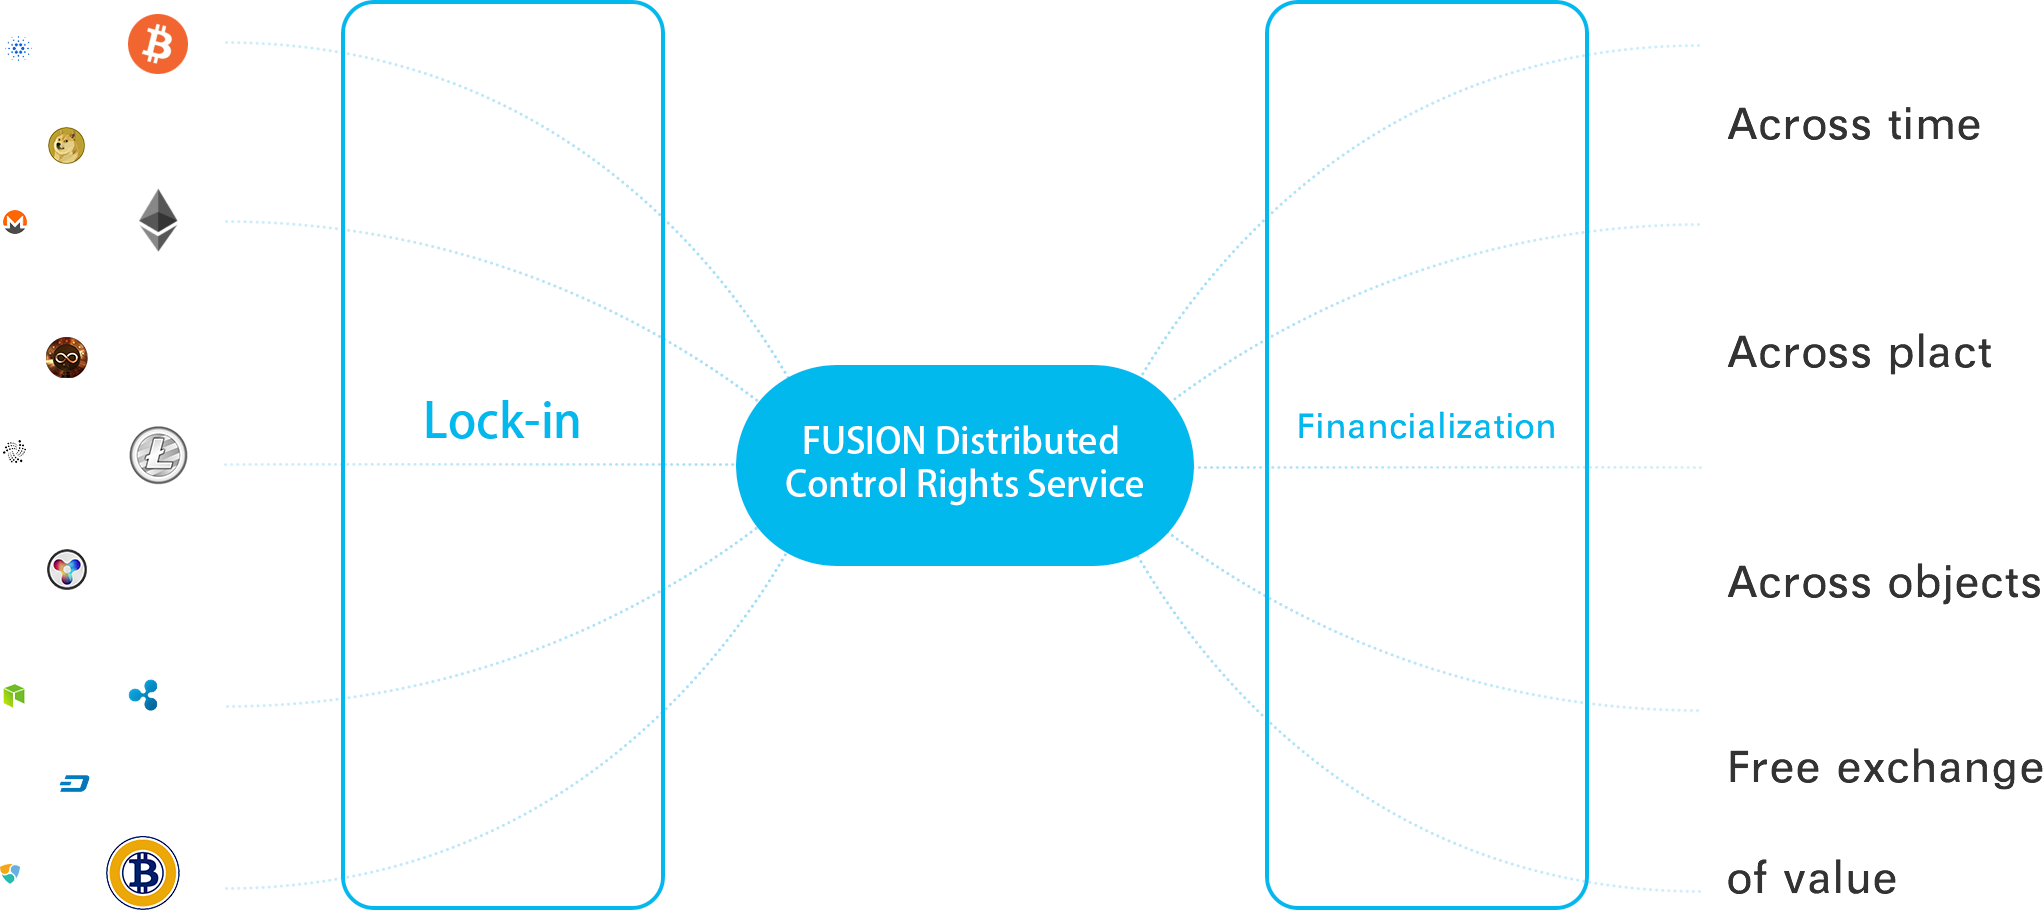
\includegraphics[width=5in]{pic/custoday.png}
	\caption{分布式控制权管理}\label{fig:1}
\end{figure}

通过对于某一种数字资产进行分布式控制权管理,使其能与其他不同种类的数字资产进行自由交互,从而使这些数字资产转化为一种金融产品,成为金融市场买卖和约定的对象。这为所有数字资产在原有功能之外增加了金融服务的功能。

\subsubsection{所有权和使用权的分离}

比特币通过简单脚本实现了两个对手之间的代币转移,以太坊通过智能合约实现了触发式的交易,但两者以及后来的区块链都只实现了通过私钥将同一种代币的所有权和使用权作为整体从一方向另一方的转移。但诸如借贷和财富管理这样的大量的金融应用要求实现使用权的暂时分离,并通过使用权交换各种其它价值形成投资组合的方式来产生收益。这使价值互联网在构建更为丰富的金融应用方面捉襟见肘。

FUSION将通过分布式矿工节点控制服务在保留所有权的情况下使各种代币的使用权转移给矿工控制,从而简单明了地实现了多种代币的所有权和使用权的分离,并且使平台上的智能合约天生地拥有了多币种的所有权和使用权分开编程的能力。这种能力接触多条件触发机制能够完成复杂的金融功能,这将在多条件触发机制时论述。

\subsection{分布式控制权管理的实现}

\subsubsection{实现的功能}

分布式控制权管理包括对数字资产Lock-in和Lock-out的两个基本步骤。在实现Lock-in的过程中,分布式控制权管理是通过原子化交易完成资产映射的。对于Lock-out,解除分布式控制权管理与解除资产映射也是如此。

不管是Lock-in还是Lock-out,其核心是如何实现数字资产原有的控制权安全稳妥地转移到非中心化的系统上,并对私钥实现可靠稳妥的保管和使用。

在Lock-in和Lock-out的实现过程中,通过运行在FUSION上对应的基础智能合约,完成目标数字资产转交到一个由分布式密钥生成算法产生的地址,实现控制权到非中心化管理的移交。

分布式控制权移交完成之后,该智能合约为用户在FUSION上的账户更新状态,以体现Lock-in或者Lock-out完成。记账的过程实际上由FUSION向用户账户发放或者收回等量数字资产的记账代币,如此就完成了数字资产到FUSION上的映射或从其上解除映射。映射对于数字资产持有者来说是透明的,只是用户存储自己数字资产的密钥采用了密钥分片和分布式存储的方式,相比原来更为安全,并且他们的数字资产可以更加便捷地参与到丰富的金融服务中。

我们将以比特币为例介绍Lock-in实现的流程。

当用户A发起一笔10个BTC的Lock-in,用户将使用钱包作为交互界面。这个钱包具有目前多币种钱包的很多功能,但它同时拥有对不同数字资产Lock-in和管理的功能。此外,钱包中还会有基于FUSION上第三方所开发的各种金融服务,可以供用户在完成Lock-in之后方便地参与。

\begin{figure}[htbp]
\centering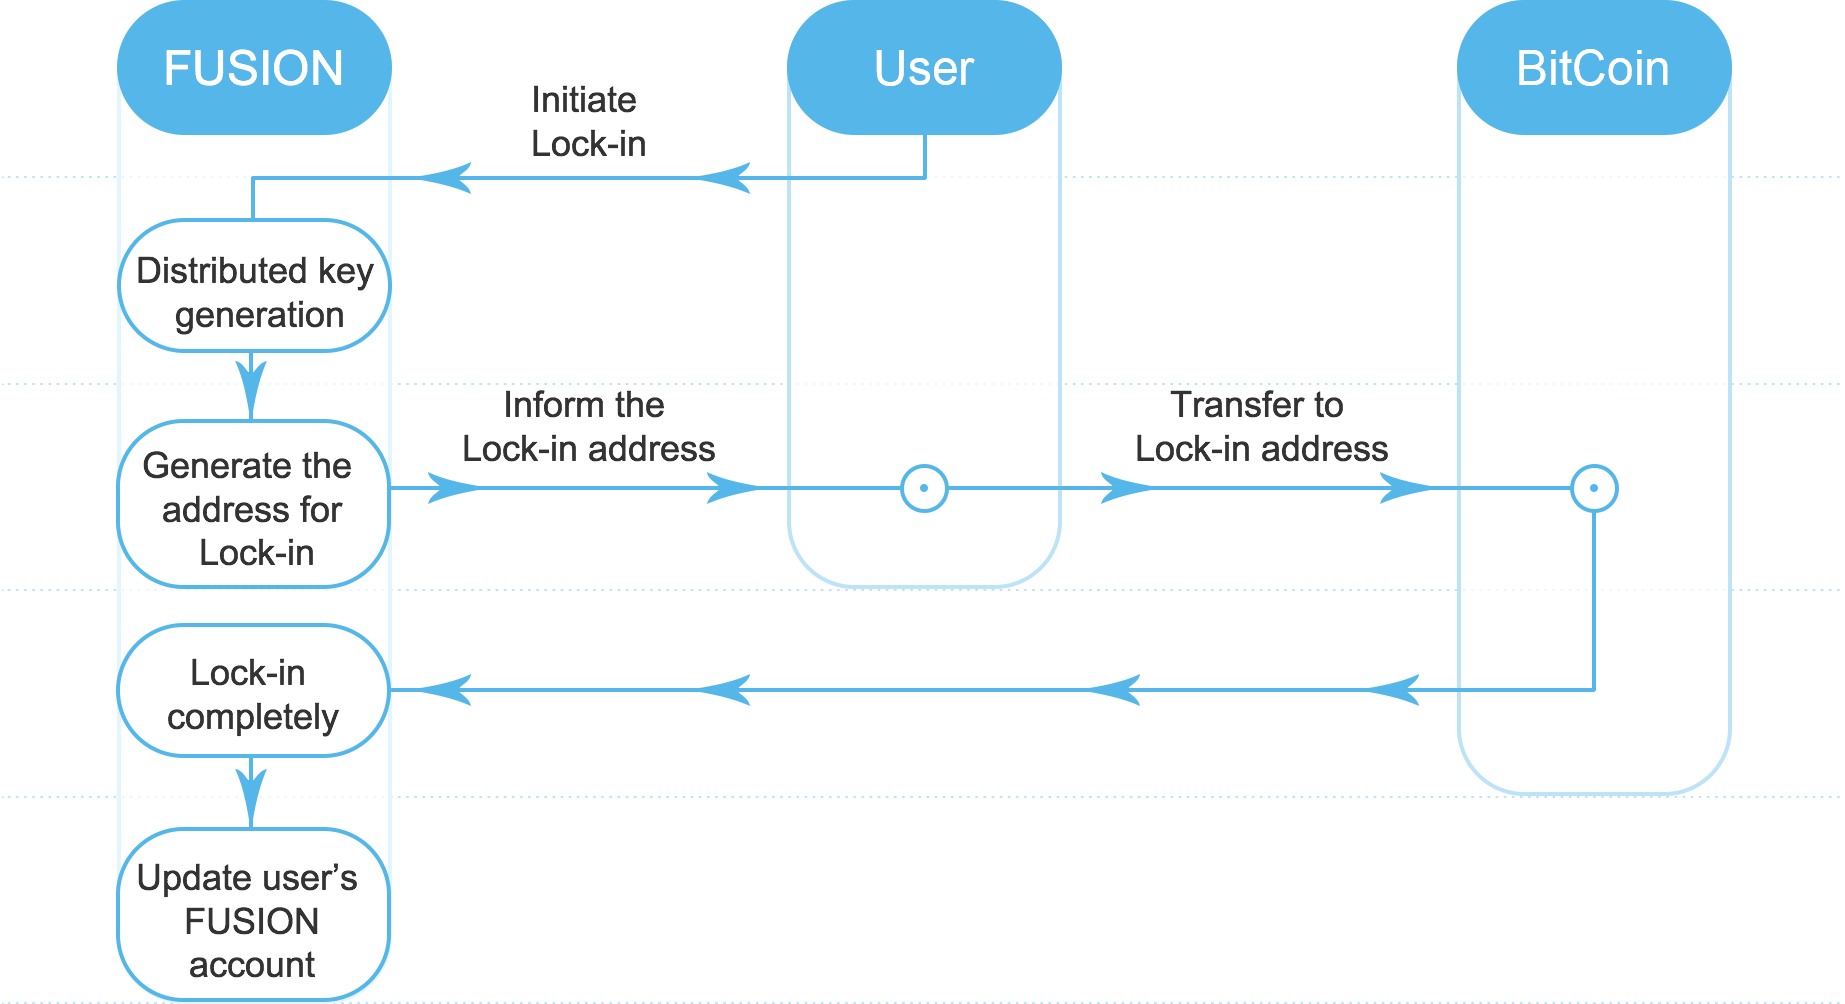
\includegraphics[width=5in]{pic/lockin.png}
\caption{Lock-in流程}\label{fig:1}
\end{figure}

\subsubsection{Lock-in的实现过程}

用户向FUSION发起Lock-in请求的体验在操作上与现有钱包转账的体验类似。具体的实现步骤如下:

(1) 发起Lock-in请求

用户A通过在钱包中调用Lock-in的程序接口,向FUSION发起10个BTC的Lock-in请求。

(2) 初始化私钥

请求操作触发FUSION上Lock-in的智能合约,由该智能合约组织私钥的初始化。所谓{\bfseries{私钥的初始化}},就是采用分布式的方式生成私钥,在这个过程中即完成了密钥分片和对分片密钥的分布式保管。私钥的初始化为今后该密钥的存储和使用奠定了基础。

(3) 移交控制权给分布式管理

初始化完成并生成位于比特币链上的一个地址,由用户A发起向该地址的转账。用户发起转账的操作经由接口在FUSION上广播本次Lock-in,由FUSION节点检查转账完成的情况。

FUSION链上的节点收到交易广播后,通过第三方接口查询该笔交易是否在比特币主链上得到确认。通过共识结果显示这10个BTC顺利转入Lock-in所生成的地址,即视为分布式控制权管理移交成功。

(4) 数字资产映射

在确认控制权移交成功之后,智能合约完成用户A在FUSION上账户的状态更新。该笔Lock-in记录由节点打包记录到FUSION的块中。至此,用户A的10个BTC的Lock-in请求完成。

\subsubsection{Lock-out的实现过程}

同样的,用户Lock-out的请求也是在钱包中通过调用相关程序接口发起的。在用户体验上与用钱包进行对外转账类似。具体实现的流程如下:

(1) 发起Lock-out请求

用户A在钱包中操作向一个链外比特币地址发起10个BTC的转账交易,即视为用户发起Lock-out请求。

(2) 检查、锁定和生成交易

该交易触发FUSION上Lock-out的智能合约,合约首先将检查用户A在FUSION上的资产状况,满足转账条件时,锁定用户A在FUSION账户中的10个比特币的状态,并生成一笔带有目标地址和用户签名的转账交易。

(3) 门限签名

FUSION链上的节点接收到交易指令,开始根据各自保存的密钥分片进行计算和比对,比对成功的节点将结果签名并进行广播。

各节点同时收集签名,当交易签名达到$t/m,\left( t \le m\right) $门限阈值的要求时,该交易由节点发送至比特币主链,实现向用户A指定的地址转账10个BTC的交易。

(4) 解除分布式控制权管理

FUSION上的节点会通过比特币对应的接口,查询该交易是否在比特币主链上得到确认。当共识得出交易确认的结果后,用户A的10个BTC将从分布式控制权管理中解除掉。

(5) 解除数字资产映射并销毁

智能合约同步更新用户在FUSION上账户的状态,通过扣减被锁定的10个BTC映射,完成映射的解除和销毁。同时,该Lock-out记录打包记录到FUSION的区块中。至此,用户本次Lock-out请求完成。

其中参与完成在跨链上发起交易、确认交易、验证交易签名的节点都将按照既定的激励机制获得相应的奖励。

\subsection{关键技术}

\subsubsection{私钥的安全性保障技术}

私钥就意味着数字资产的控制权。因此在整个过程中,如何确保私钥的有效生成,保管和使用的过程中不泄露,是安全可靠地实现数字资产Lock-in的关键性问题。由此引出对如下问题:

(1) 如果私钥完整的存储在一个地方,将会因为节点攻击或者恶意节点收集出现私钥泄露的情况。因此,FUSION为了确保私钥的安全,选择将私钥分片并交由不同的节点保管。

(2) 私钥在生成过程中不能完整的出现再进行分片,所以要实现私钥的分布式生成。

(3) 私钥在使用过程中,例如生成原链上的有效地址,,私钥或私钥分片都不能在节点间传递,以避免被恶意节点有意识地收集。同样的,私钥也不能通过组装完整后进行计算,任何私钥完整出现都可能带来泄露的隐患。这些问题需要通过分布式密码计算和门限密码系统方面的研究加以解决。

因为不同区块链有差异,不同加密数字货币之间的“分布式密钥初始化”在具体实现上会具有一定的区别。我们将在分布式控制权管理的实现和安全等领域持续进行相关研究。以下,我们将重点讨论有效生成私钥的问题。

\begin{figure}[htbp]
\centering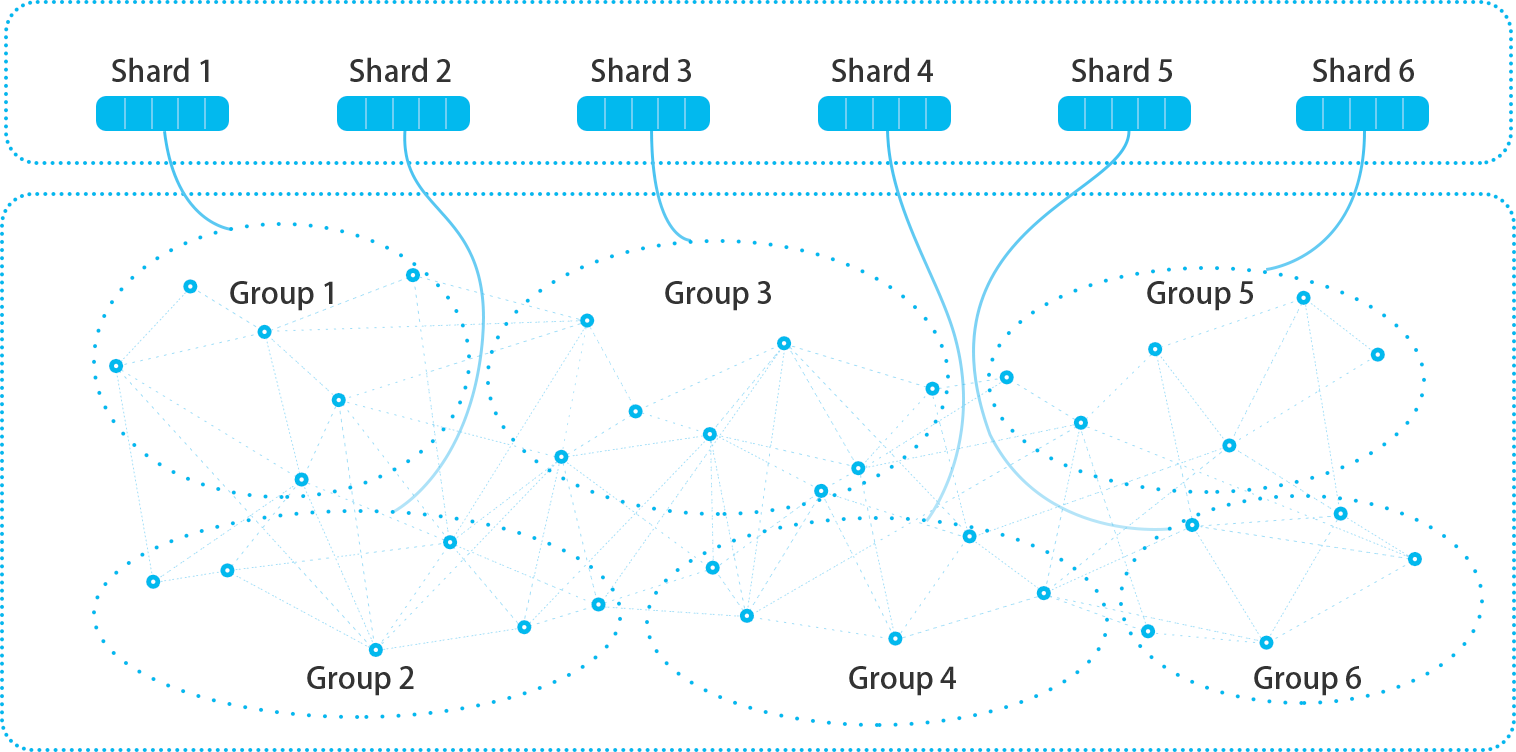
\includegraphics[width=5in]{pic/keygeneration.png}
\caption{分布式密钥生成}\label{fig:1}
\end{figure}

(1) 私钥的分布式生成

私钥的分布式生成,是通过FUSION上多个节点分布式地开展完成的,每个节点只生成并保存私钥的一部分,彼此之间并不发生私钥分片的传递和组装。

这个过程中,会根据密钥分片的算法确定分片的数量,按照这个数量形成虚拟的节点组进行私钥的生成。为了保证分布式保管的密钥一直处于可用状态,节点组的节点数量的生成算法将确保有足够多节点同时不在线的概率在一个极小的范围之内。

分片按照确定的分片长度由组中节点独立随机生成并依照既定的共识机制最终形成分片的值。

(2) 私钥的计算

私钥的使用是通过分布式密码计算来实现的。当一笔需要签名验证的交易被广播出来,节点可以根据自己保存的分片进行计算和比对。当比对成功,节点对其分片验证结果签名并广播出去。这个过程中,每一个分片结果是不可逆的,因此,无法通过广播的任何内容反推出密钥或者密钥分片。

目前,FUSION团队通过代码分析的方法,得出了hash256、椭圆曲线算法能够支持私钥分片生成和分布式计算的结论。对于有些原链采用了不支持分片计算的算法,将考虑采用同态加密的方法,实现在密钥不泄露情况下对密钥的计算。

(3) 交易确认

节点在完成私钥分片验证的同时,通过广播收集分片签名的结果,当一笔交易的分片签名达到一个门限值时,该交易就被认为有效。

\subsubsection{分布式密钥生成}

FUSION采用的密码共享\citep{Feldman1987}使用了分布式密钥生成协议(Distributed Key Generation,简称DKG)的相关理论和成果。由n个节点共同合作生成通信中的公钥和私钥,公钥以公开的形式广播,私钥通过可验证秘密共享协议(Veriable Secret Sharing,简称VSS)以分片的方式由各节点单独保存。通过DKG算法生成公共的公钥,进而以相应算法生成Lock-in的账户地址,实现控制权的分布式管理。

在这里引用了VSS-DKG领域基于椭圆曲线密码的分布式密钥生成协议和应用\citep{Wang2007}方面的研究对相关过程介绍如下:

已知椭圆曲线$E$,存在有限域$GF(q)$,$q$为素数,有$n$个参与者集合$Q = \left\{ {{P_1},{P_2},...,{P_n}} \right\}$,${p_i}$表示第$i$个参与者$P_{i}$的身份,且${P_i} \in G{F^*}\left( q \right)$,其中$G{F^*}\left( q \right)$是$GF\left( q \right)$上的乘法群。同时${p_i}$和$i$在计算过程中可以互换,$E/GF\left( q \right)$表示$E$上的加法群,$T$是$E/GF\left( q \right)$上的基点,$E/GF\left( q \right)$的阶为素数或为素数因子,记这个素数或素数因子为$p$。

在该密钥生成协议中,假设标量乘法及点乘都是在$\delta $上完成的,其它运算都是在$GF\left( q \right)$上完成的。为了计算$Q\left( x \right)T$,先计算$Q\left( x \right)$,然后对$Q\left( x \right)$取模$p$运算,即$Q\left( x \right)\bmod p$,而$Q\left( x \right)\bmod p$就是点$T$上的标量乘法。

再假设$\delta $上的椭圆曲线$E$有另一个基点$T'$。

接下来是对于DKG协议的描述:

(1) 生成私钥${s_i}$:

a) $p_{i}$随机选择$2t+2$个数,$a_{ik}\in GF(q)$和$b_{ik}\in GF(q), k=0,...,t$,$a_{ik}$,$b_{ik}$作为次数为$t$的多项式的系数:

\begin{equation}
  \label{eq:TA}
  f_i(z)=a_{i0}+a_{i1}z+...+a_{it}z^t
\end{equation}

\begin{equation}
  \label{eq:TA}
  f_i(z)=b_{i0}+b_{i1}z+...+b_{it}z^t
\end{equation}

i. $p_i$计算:
\begin{equation}
  \label{eq:TA}
 s_{ij}=f_i(p_i) \bmod \ p
\end{equation}

\begin{equation}
  \label{eq:TA}
 {s_{ij}}' = f{'_i}\left( {{p_j}} \right)\bmod p,j \in {S_i}%s_{ij}=f_i(p_i)\bmod \ p, j \in S_i
\end{equation}

ii. $p_i$计算t+1个公开值:${P_{ik}} = \left( {{a_{ik}}T} \right) \oplus \left( {{b_{ik}}T'} \right),k = 0,...,t$

b) 秘密信息的分发:$p_i$通过自己与$p_j$之间的保密信道发送包含$s_{ij}$和${s_{ij}}'$的消息给$p_i,j\in S_i$。

c) 公开信息的分发:$p_i$广播包含$\left\{ {{P_{ik}}|0 \le k \le t} \right\}$的消息。

d) $p_i$收到由$p_j$发送来的$s_{ji}$和${s_{ji}}'\left( j\in S_i\right) $,对于$j\in S_i$的参与者,执行如下操作:

i. 通过下式进行验证:
\begin{equation}
  \label{eq:YZ}
\left( {{s_{ji}}T} \right) \oplus \left( {{s_{ji}}'T'} \right) = \sum\limits_{k = 0} ^t {} ^\oplus  p_i^k{P_{jk}}
\end{equation}

ii. 如果\ref{eq:YZ}式验证失败,则$p_j$向$p_i$发送一个抱怨。

iii. 如果$p_i$收到来自$p_j$的抱怨,$p_i$重新广播$s_{ji}$和${s_{ji}}'$使其满足\ref{eq:YZ}式。

e) 如果存在如下两种情况,就更新$s_i$,${s_i} = \sum\limits_{}^{} {_{j \in {Q_i}}{s_{ji}}} $

i. $p_j$收到$t+1$个或更多个不同的抱怨,则需更新$s_i$。

ii. $p_j$再次广播$s_{ji}$和${s_{ji}}'$,但是收到的$s_{ji}$和$s_{ji}^{'}$仍然无法满足\ref{eq:YZ}式,则需要更新$s_i$。

(2) 生成公钥$y_i$:

a) 计算$A_{i0}=a_{i0}T$并广播$A_{i0}$。

b) 收到$A_{j0}$并计算公钥${y_i} = \sum\limits_{j \in {Q_i}}^{} {^ \oplus } {A_{j0}}$

以上DKG协议的安全性证明可参考\cite{Gennaro1999}的研究。
	
\subsubsection{门限签名}

区块链是一种非中心化、自组织的分布式网络,节点之间无信任关系,可以自由加入和退出。FUSION进行分布式签名的过程中,如果拥有私钥某一个分片的节点退出网络则会导致签名失败,出现无法完成交易等问题。FUSION链采用$\left( t,m\right) ,t \le  m$的门限签名方案\citep{Shamir1979}。在$m$个节点组成的链中,链中任何不少于$t$个节点合作就能完成签名。

\begin{figure}[htbp]
\centering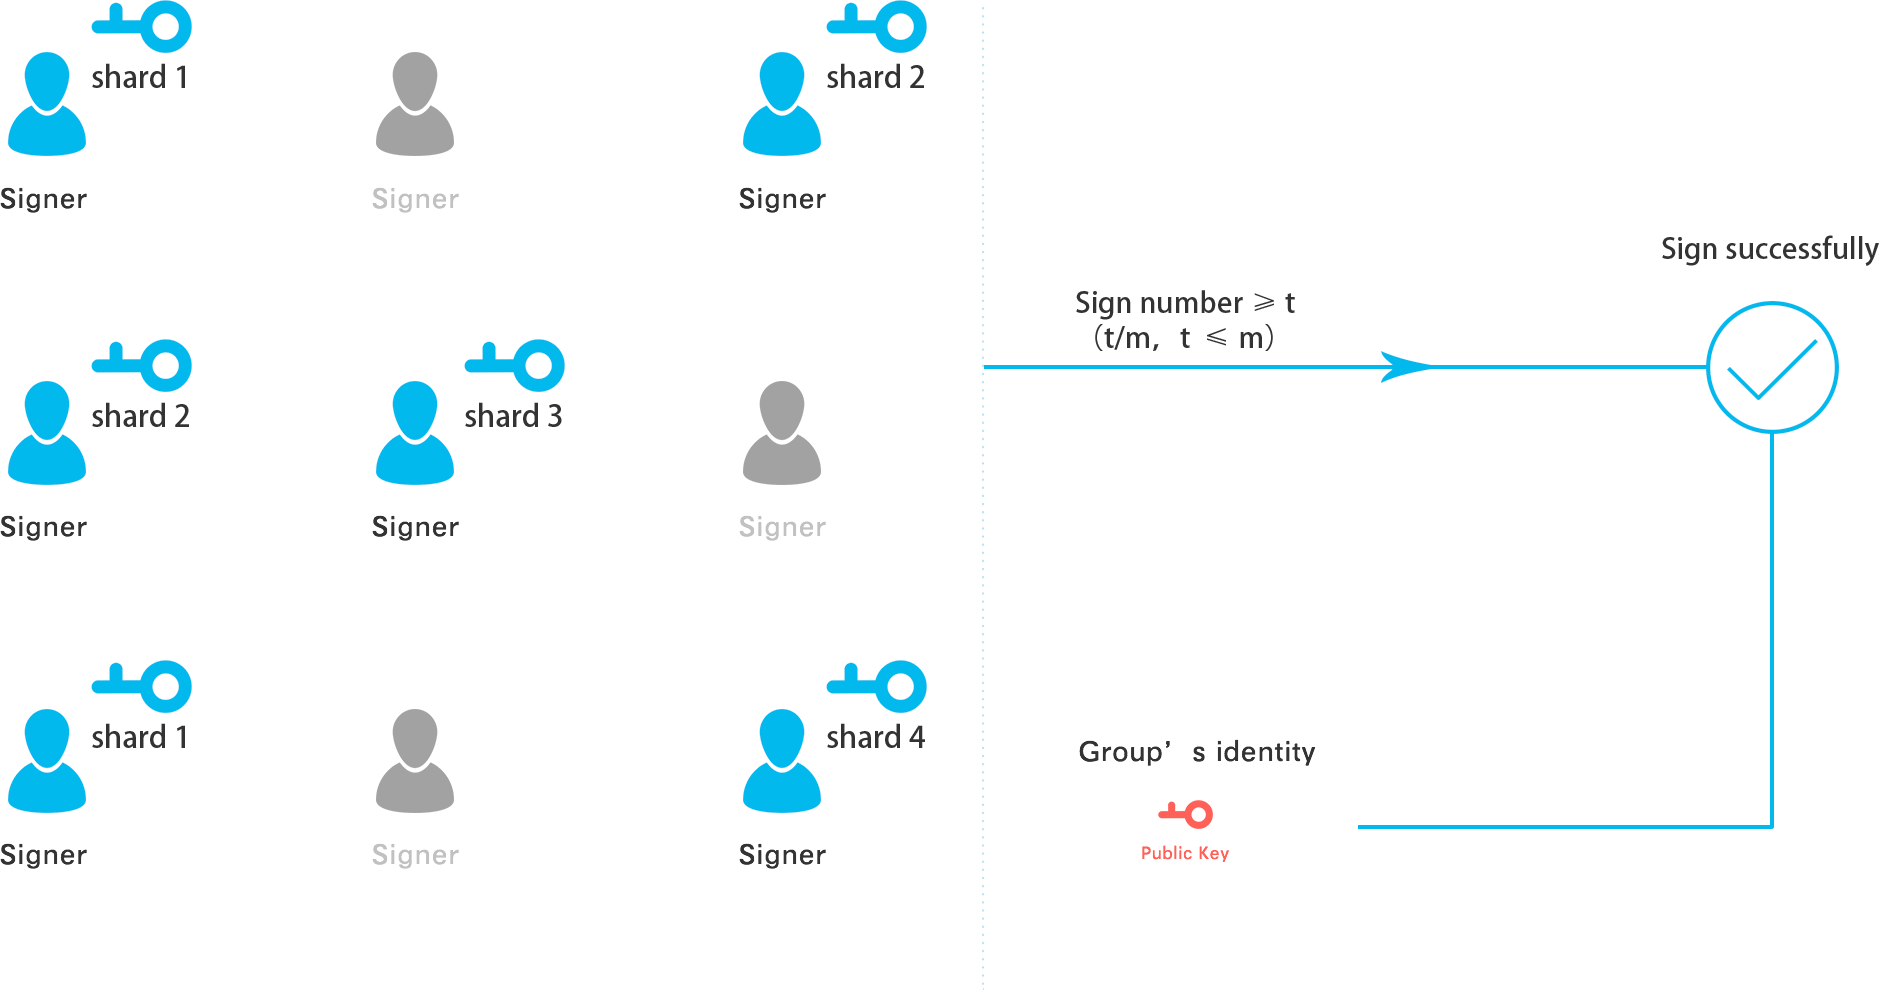
\includegraphics[width=5in]{pic/thresholdsign.png}
\caption{门限签名}\label{fig:1}
\end{figure}

门限签名可以解决FUSION链节点退出导致签名失败的问题并且可以提高区块链网络的稳定性。根据对于分布式密钥生成网络中节点进出的自适应方面的研究成果\citep{Zhajun2010},对于极端情况下,FUSION链会选择候选节点加入并刷新共享密钥参数,保证FUSION链的有效运行。

\section{加密金融智能合约}

\subsection{定义多方之间的金融关系}

\subsubsection{对智能合约的增强}

所谓{\bfseries{加密金融智能合约(Cryptofinancial Smart Contract,CSC)}},是指用于界定一种或多种数字资产在多个参与者之间、在时间继起和空间位置上的关系和价值交互条件,从而实现一种或多种数字资产在多种参与者之间进行金融交易的智能合约。

这里的数字资产是指不同数字资产Lock-in之后,在FUSION链上映射的资产。从而使得FUSION上的智能合约可以同时对多种不同的数字资产间的关系进行定义。

多个参与者是指不同数字资产的所有者和使用者。在FUSION链上以账户形式体现的,包括用户账户和合约账户。在加密金融智能合约中,合约对象可以包括多个用户账户以及多个合约账户。

因为金融的本质是跨越时间和跨越空间的价值交换,通过智能合约对金融交易进行描述时,就转变为对于不同数字资产、不同所有权和使用权在时间和空间关系上的描述。

现有的智能合约,存在如下限制:

\begin{itemize}[itemindent=1em]
	\item 只能对同一条链上的两个对手之间的同一种数字资产进行操作;
	\item 只能对数字资产所有权进行转移,数字资产的使用权和所有权不可分割的;
	\item 只能以交易触发,缺少链外触发条件以及有效的链外信息输入。
\end{itemize}

这些限制影响了在现有的区块链和智能合约上实现复杂金融交易的可能性。因此加密金融智能合约的增强将体现在:

\begin{itemize}[itemindent=1em]
	\item 实现多方之间,多种数字资产间所有权和使用权的应用;
	\item 增加多种触发机制;
	\item 实现有效的链外数据输入;
	\item 通过智能合约对智能合约的嵌套调用,体现智能合约自身的金融属性。
\end{itemize}

\subsubsection{加密金融功能}

对数字资产的分布式控制权管理已经实现了不同数字资产之间的交互,成为FUSION上加密金融智能合约可以定义和编程的对象。因此有条件也有必要通过加密金融智能合约实现多角色、多币种、使用权分离的加密金融应用。

{\bfseries 多角色}是指一个加密金融智能合约具有同时支持多个不同账户类型的能力,可以定义多个用户之间以及多个智能合约之间的关系。

{\bfseries 多币种}是指通过Lock-in将不同的数字资产映射到FUSION上之后,可以由FUSION上的智能合约同时对多个不同种类的数字资产之间的关系进行定义。

{\bfseries 使用权分离(Separation of Use Rights )}是指数字资产使用权与所有权可以分离。目前的智能合约只能实现代币的转移,无法做到一个对象保留所有权的同时由另一方获得该笔数字资产使用权,即所有权与使用权是一体的。而在加密金融智能合约中,一个合约里可以同时定义两个以上用户账户和两个以上的合约账户,也就有条件实现数字资产的所有权和使用权的分别定义,从而很容易地实现诸如不同数字资产间抵押借贷等金融交易。

\begin{figure}[htbp]
\centering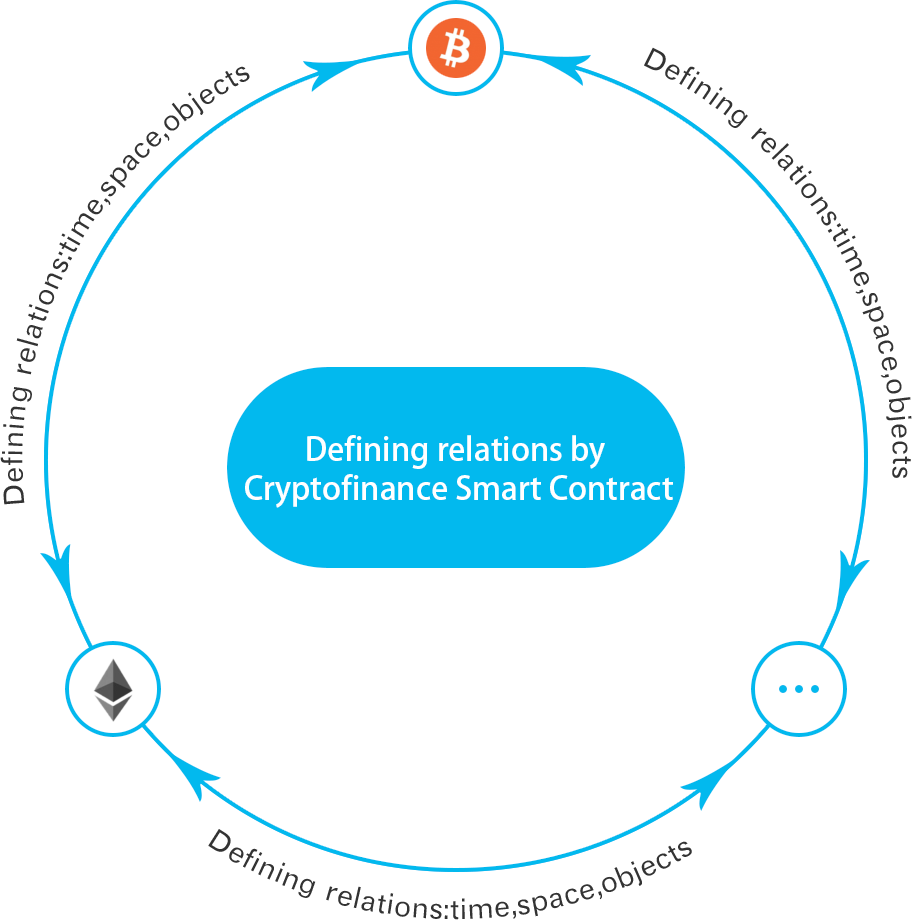
\includegraphics[width=4in]{pic/financialization.png}
\caption{金融关系界定}\label{fig:1}
\end{figure}

图 \ref{fig: frd} 显示了加密金融智能合约如何实现不同数字资产进行关系定义。位于图中三个顶点的是对不同种类数字资产在FUSION上的映射。通过智能合约,在它们彼此之间同时建立起关于时间、空间以及使用权、所有权关系的定义。这些定义将在某些条件触发的情况下,按照合约中预置的操作对其中部分或者全部进行操作。这些触发条件可以是一笔主动的交易,也可以是时间条件,或者是一个事件的发生。

如果数字资产之间的关系仅以空间定义,那么就实现了不同数字资产之间的转移。如果以时间定义,就构成了p它们之间的借贷关系。如果以所有权和使用权进行定义,就体现了不同数字资产之间所有权和使用权的关系。由此可以看到,通过对不同时间、空间和对象间一种或多种关系的逻辑定义,就可以实现在不同数字资产之间构建从简单到复杂的金融交易,甚至包括实现目前还没想到的金融创新,形成无限的想象空间。

\subsection{合约的多种触发机制}

\subsubsection{触发条件的多样性}

目前智能合约实现的应用是以数字资产所有权的转移为基础的,这是由于当前智能合约是以一笔向该合约的转账交易触发的。

例如,以太坊的智能合约如图\ref{fig:SCOM}。

\begin{figure}[htbp]
\centering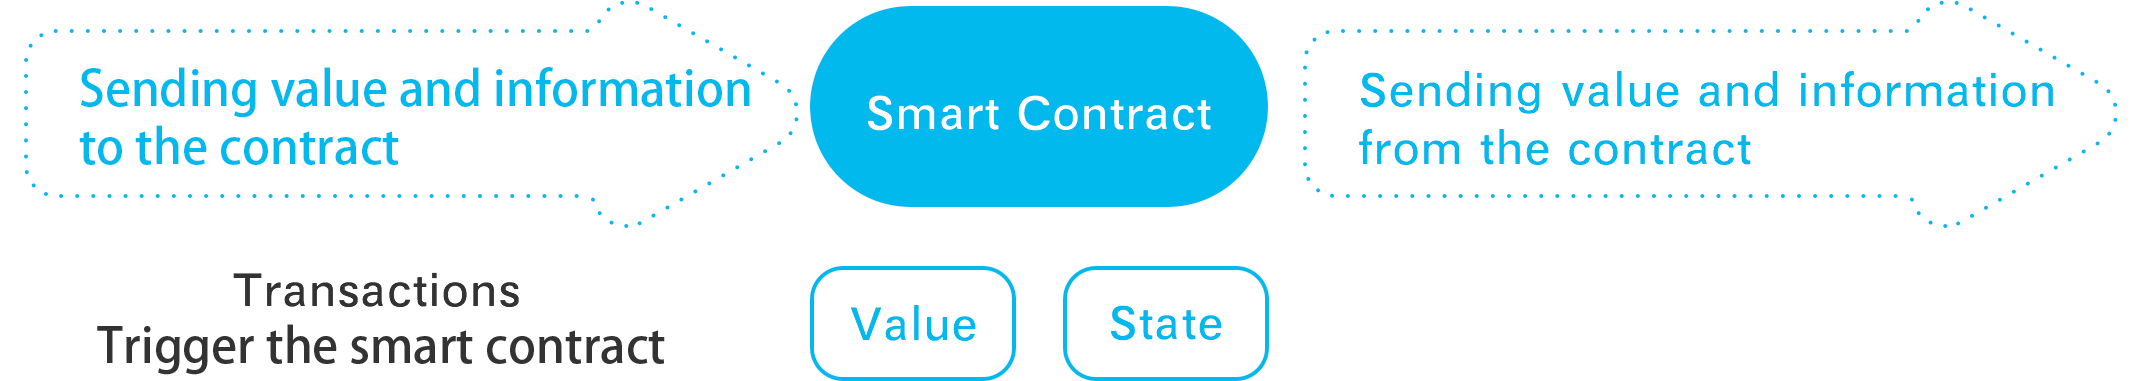
\includegraphics[width=5in]{pic/singletrigger.png}
\caption{智能合约单触发机制}\label{fig:1}
\end{figure}

在这里,通过向一个智能合约地址发起一笔交易,从而触发这个智能合约在节点虚拟机上的执行,这样的触发模式称之为主动触发。

以实现募捐的智能合约举例说明,当一个用户向该智能合约发起一笔转账交易,合约首先核对这笔转账交易的有效性,包括核实用户帐户是否金额。然后,智能合约调用相应的接收募捐的函数,并按照函数中预置的响应条件,例如募捐总额的条件,进行判断,总额未满则接收该笔捐款。最后,合约将改变后的智能合约的合约值(Value和State)写进区块中以记录发生过该笔募捐交易。

从以上分析我们看到,智能合约中的函数会包含对于一些条件的判断,但是如果没有一笔转账交易先行触发智能合约,这些预置条件是不会对这些条件进行判断的。即使相关条件满足,也不会触发智能合约中后续规则的执行。如果智能合约不能由除交易之外的外部条件主动触发并执行,很多金融交易场景,比如被动式的量化交易策略,就没办法实现。所以,加密金融智能合约首先要增强触发机制,除了支持现有的主动触发机制,还扩充了定时触发和事件触发的两种触发机制。我们称扩展后的触发机制为{\bfseries 多触发机制(Multiple Triggering Mechanisms)}。

\begin{figure}[htbp]
\centering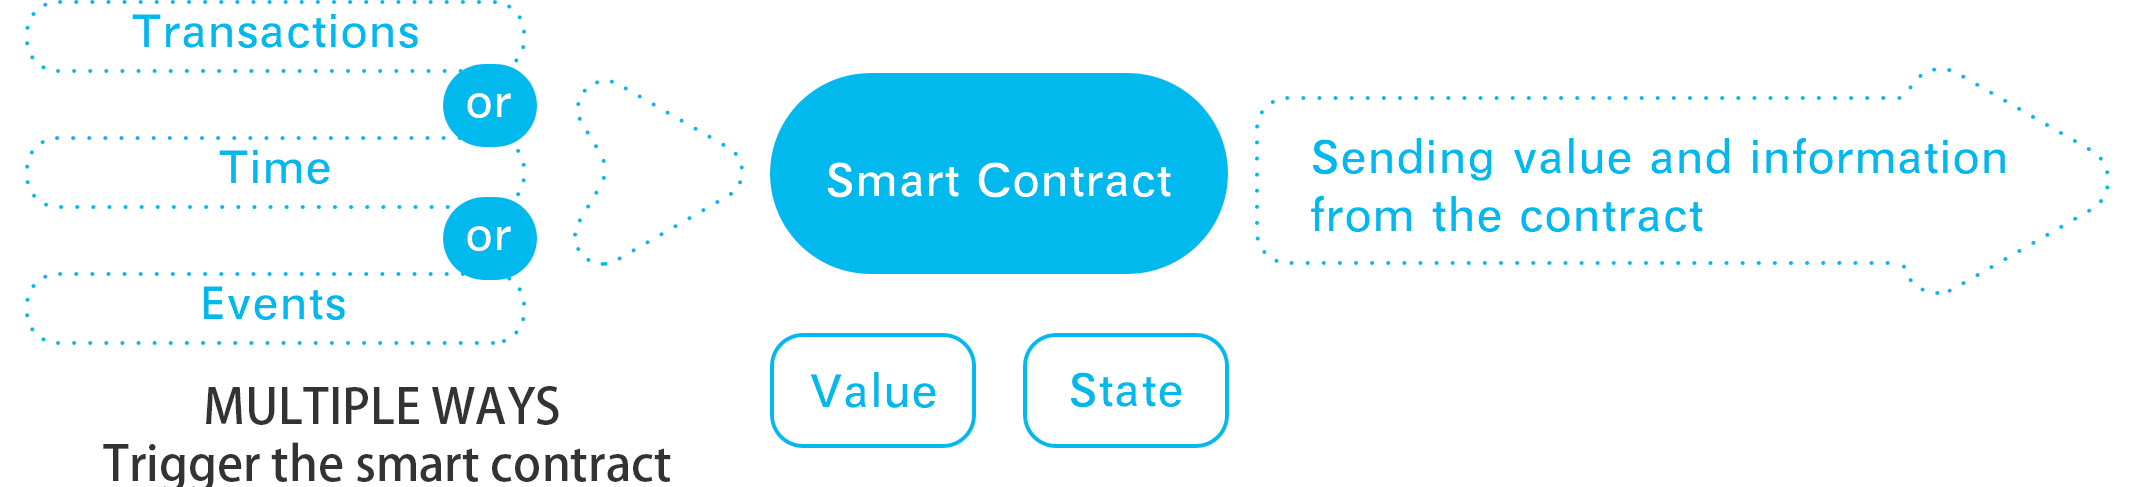
\includegraphics[width=5in]{pic/multipletrigger.png}
\caption{加密金融智能合约多触发机制}\label{fig:1}
\end{figure}

多触发机制包括以下三种触发方式:

\begin{itemize}[itemindent=1em]
	\item 主动触发方式与现有的智能合约触发方式一致,现有各类智能合约都被支持。
	\item 定时触发方式,是指智能合约将被时间条件触发招待,比如时间点或时间长度。例如借贷场景就是典型的跨时间的互换,这样的应用将受到时间触发方式的很好地支持。
	\item 事件触发方式,是指当发生某个事件时,智能合约将被触发执行。例如,在自动化交易、量化交易中,对于事件的捕捉是相当重要的,这样的应用场景就需要用到事件触发方式。
\end{itemize}

以上三种触发机制是通过抽象各类应用场景形成的,能够满足复杂加密金融应用中对于智能合约触发调用的各类需求。

\subsubsection{链外信息输入}

目前,智能合约所能处理的信息来源于所在区块链系统的内部,而要实现了智能合约多种触发机制,部分触发信息将源于链外。因此,加密金融智能合约将构建链外信息输入接口(External Information Input Interface),并通过相应机制确保链外信息的有效和真实性。

首先,FUSION会基于第三方数据源提供的标准的API接口,通过http或者socks的途径由节点获得相关数据。FUSION会对一些常用的链外数据源的数据调用进行封装,实现类似于system call的方式供应用或者节点获取数据。实际上,节点也可以利用上述的数据获取渠道创建自己的数据源来获取相关的数据信息。

链外获取数据的真实性是由共识机制判断的。当一个节点发现某个智能合约的触发条件相关的链外数据的满足条件时,节点触发智能合约。假如一个恶意节点故意向全网广播某个智能合约满足触发条件,但其他诚实的节点在执行时还将验证,因此很容易在智能合约执行的过程中发现条件不符合而终止执行。这样的恶意行为不会对智能合约的实际运行产生任何破坏作用,也不会存在作恶获利的可能性。

激励机制也有助于解决了链外输入数据源有效性的问题。这是因为数据成功确认需要全网共识,节点只有设法找寻更快更可靠的数据源并争取正确验证触发条件,才能为其带来更多收益。通过市场有效性和资源分配,高效率的节点会受到奖励。少数恶意节点捏造的不真实的数据难以影响最终的数据真实性。

\subsubsection{兼容与增强实现}

FUSION上加密金融智能合约,将在以太坊智能合约的基础上进行增强与开发。对于诸如触发机制等的增强,将在兼容现有的以太坊智能合约的基础上实现功能扩展。这将使得现在运行在以太坊上的智能合约能够简单地迁移到FUSION上,也能够使得现在智能合约的开发者快速地实现在FUSION上的开发。

下一个阶段,会优化编程语言和虚拟机,实现更丰富的应用开发环境,并将面向那些几乎没有代码经验的应用开发者提供更直观易用的应用开发工具和调试环境。

\subsection{合约的嵌套调用}

以上对现有智能合约的功能增强,最终使得FUSION上的智能合约能够完成在不同条件下,对不同价值、不同对象,在时间和空间上的关系和交互规则的定义,从而使得FUSION上的智能合约能更加灵活地构建金融应用。

FUSION上智能合约的输出不仅能实现对于账户状态和值的更新,还可以在一个智能合约执行的过程中实现对另一个智能合约满足一定条件下的调用。

实现智能合约A对智能合约B的调用,需要完成以下的工作:

(1)构建调用的智能合约

在智能合约A的代码中,增加对于调用智能合约B的预置条件判断和预置条件规则,并且增加目标智能合约地址索引的参数。条件判断的依据来源于智能合约A触发时的数据输入,以及基于这些数据计算得到的结果。在预置条件满足的情况下,节点将下载智能合约B进行执行。

调用条件的描述包括判断规则和时间规则两部分内容。判断规则是事先写入合约的计算函数。时间规则可以一个每一次执行一个合约时都被触发的预置条件,也可以是一个周期性检查智能合约A状态的定时条件。

(2) 嵌套调用的实现过程

i. 智能合约A被触发执行时,按照预置的嵌套调用条件执行函数,对是否调用智能合约B进行判断。

ii. 调用条件满足时,执行预置的计算函数,计算生成需要输入智能合约B的数据结果。

iii. 由执行智能合约A的节点下载智能合约B到本地运算环境,将上一步骤计算得到的数据作为智能合约B的数据输入,开始执行智能合约B。

通过以上步骤完成智能合约A在执行过程中对智能合约B的调用。由于智能合约B是以智能合约A的状态作为触发调用的判断依据,并且会基于智能合约A对其输入的不同数据执行不同的操作,从而建立其两者的调用逻辑关系,因此称为嵌套调用。

智能合约不仅对各自合约内的业务逻辑进行判断,还将通过预置条件调用其它智能合约。这样就容易构建起不同智能合约之间的网络状调用关系,这使相互关联的金融应用之间建立起了价值交互关系,从而为创造复杂的应用逻辑提供了可能。因此,通过智能合约之间的嵌套调用功能,可以构建复杂的金融服务,例如对应于以现金流作为依据的借贷应用。

\subsection{合约的开发}

\subsubsection{合约的编写与发布}

为了实现面向金融的智能合约,需要完成以下步骤:

(1)创建一个智能合约

FUSION上发布的智能合约是对现有智能合约的扩展。创建的智能合约应该包括定义和描述两部分。

其中的定义部分与现有的以太坊的智能合约一致并兼容。它包含了合约状态、合约值,以及预置响应条件和响应规则的函数代码。因此,现有以太坊上的智能合约在FUSION上是兼容的。

描述部分包含了对于这个智能合约所要采用的触发描述:选择定时或者条件(事件)的触发机制、轮询时间、信息源等。

\begin{figure}[htbp]
\centering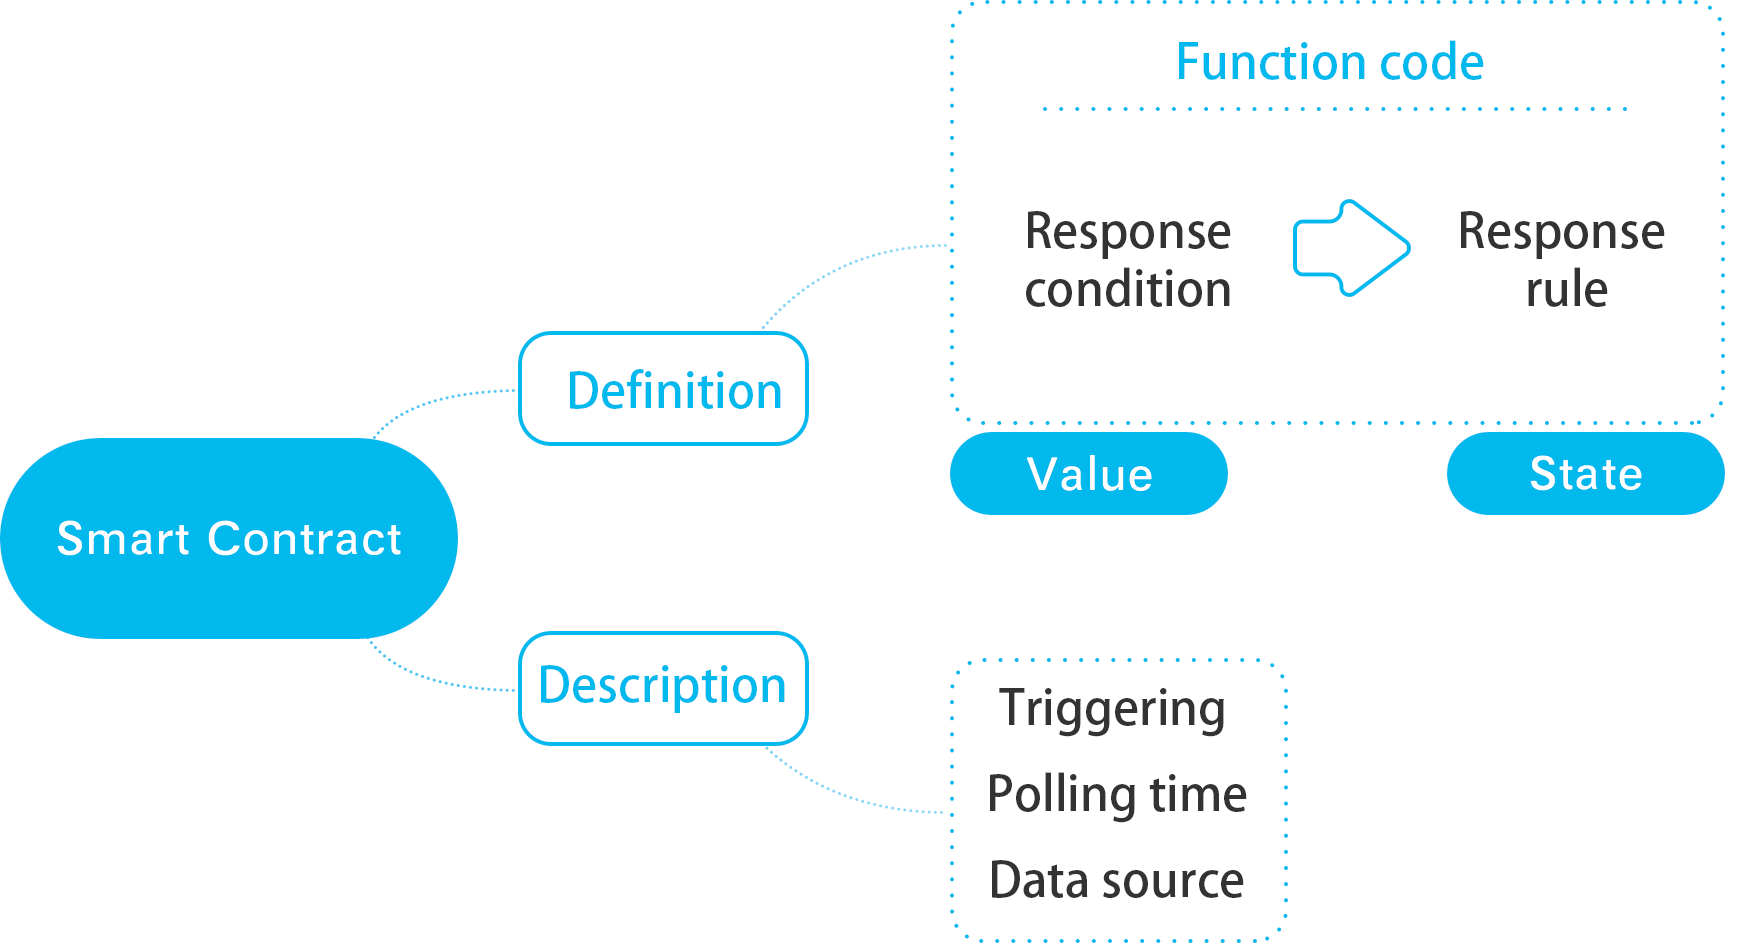
\includegraphics[width=5in]{pic/CFSC.png}
\caption{加密金融智能合约编写}\label{fig:1}
\end{figure}

(2)发布一个智能合约

智能合约发布之后,定义部分的存储与现有的智能合约在区块链上的存储方式一致。而描述部分会与当前区块链上所有智能合约的触发条件合并形成一个触发条件列表(Calling list),这个列表被存储到区块里供全网访问。

在列表中,每一行记录对应一个智能合约,每一条记录除了描述中所包含的内容之外,还包括对应智能合约存储的索引地址。


\begin{figure}[htbp]
\centering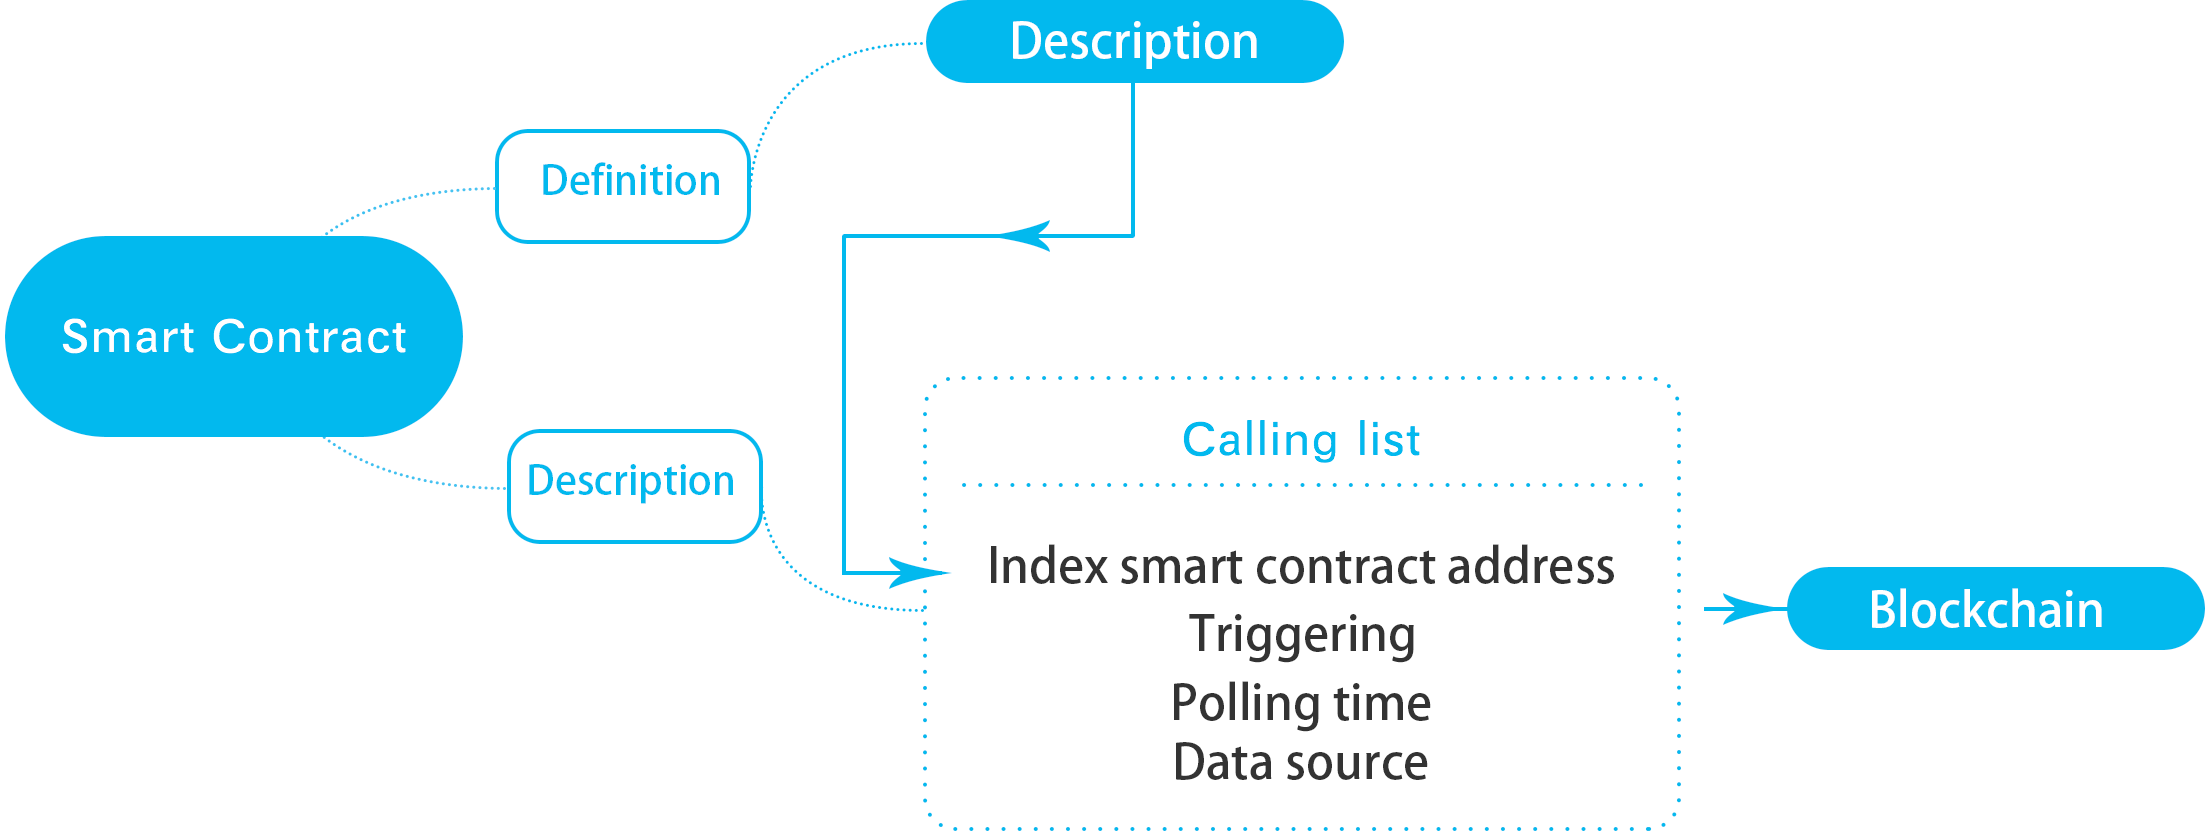
\includegraphics[width=5in]{pic/CFSCre.png}
\caption{加密金融智能合约发布}\label{fig:1}
\end{figure}

\subsubsection{定时和条件触发的实现}

主动式的触发与现有以太坊上智能合约的触发方式一致,由一笔向合约地址的转账触发。对于新增的定时触发和条件(事件)触发的实现将通过以下几个步骤实现:

(1)节点对触发条件进行判断

触发条件列表(Calling list)由被下载到本地进行执行。节点对列表进行轮询,从对应的或者节点自有的数据源获得相关数据并判断是否满足触发条件。

(2)触发智能合约的触发

记账节点在某一时刻的轮询中,发现某个智能合约的条件满足,则根据触发条件列表(Calling list)中对应的智能合约地址索引获取该智能合约地址并向该地址发送一个指定交易以实现对该智能合约的触发。同时,全网记账节点也通过这个指定交易,下载该智能合约进行执行。

(3)执行智能合约

智能合约的执行方式与目前智能合约的执行方式一致,即在节点的运行环境(虚拟机)中执行。不同的是,合约中包括了新的触发条件并可以通过触发条件嵌入其它合约,从而形成事件的链。
	
\subsubsection{接口与快速开发}

FUSION将提供智能合约的编程环境和函数库。开发者可以通过调用这些函数,实现智能合约的快速开发。开发环境将封装各种区块链、智能合约、数据源等作为接口,以使数据的获取和交互更加便捷。

以下是几种典型的调用接口分类:

(1)密钥管理

实现与密钥有关的相关功能,包括:

\begin{itemize}[itemindent=1em]
	\item 初始化密钥对,生成并返回公钥地址。
	\item 输入公钥地址和对应的签名,返回签名的hash值。
\end{itemize}

(2)区块链数据获取

如果将区块链看成支撑分布式应用DApp运营的系统,智能合约对区块链数据的获取相当于获取所在区块链系统的全局变量。通过此类接口,智能合约可以获得如下存在于区块链上的信息:

\begin{itemize}[itemindent=1em]
	\item 目标块高度。
	\item 发送者信息。
	\item 接受者信息。
	\item ... ...
\end{itemize}

(3) 对智能合约的调用

由于FUSION上的所有功能通过智能合约实现的。比如,在一个智能合约里实现转账,实际上是通过调用转账智能合约完成的。FUSION将用更加基础的智能合约对具有共性的金融应用进行封装。因此,在FUSION编写智能合约的过程就是,不断调用更加基础的智能合约形成常用金融应用的过程,并以此构建更加复杂的功能。

\begin{figure}[htbp]
\centering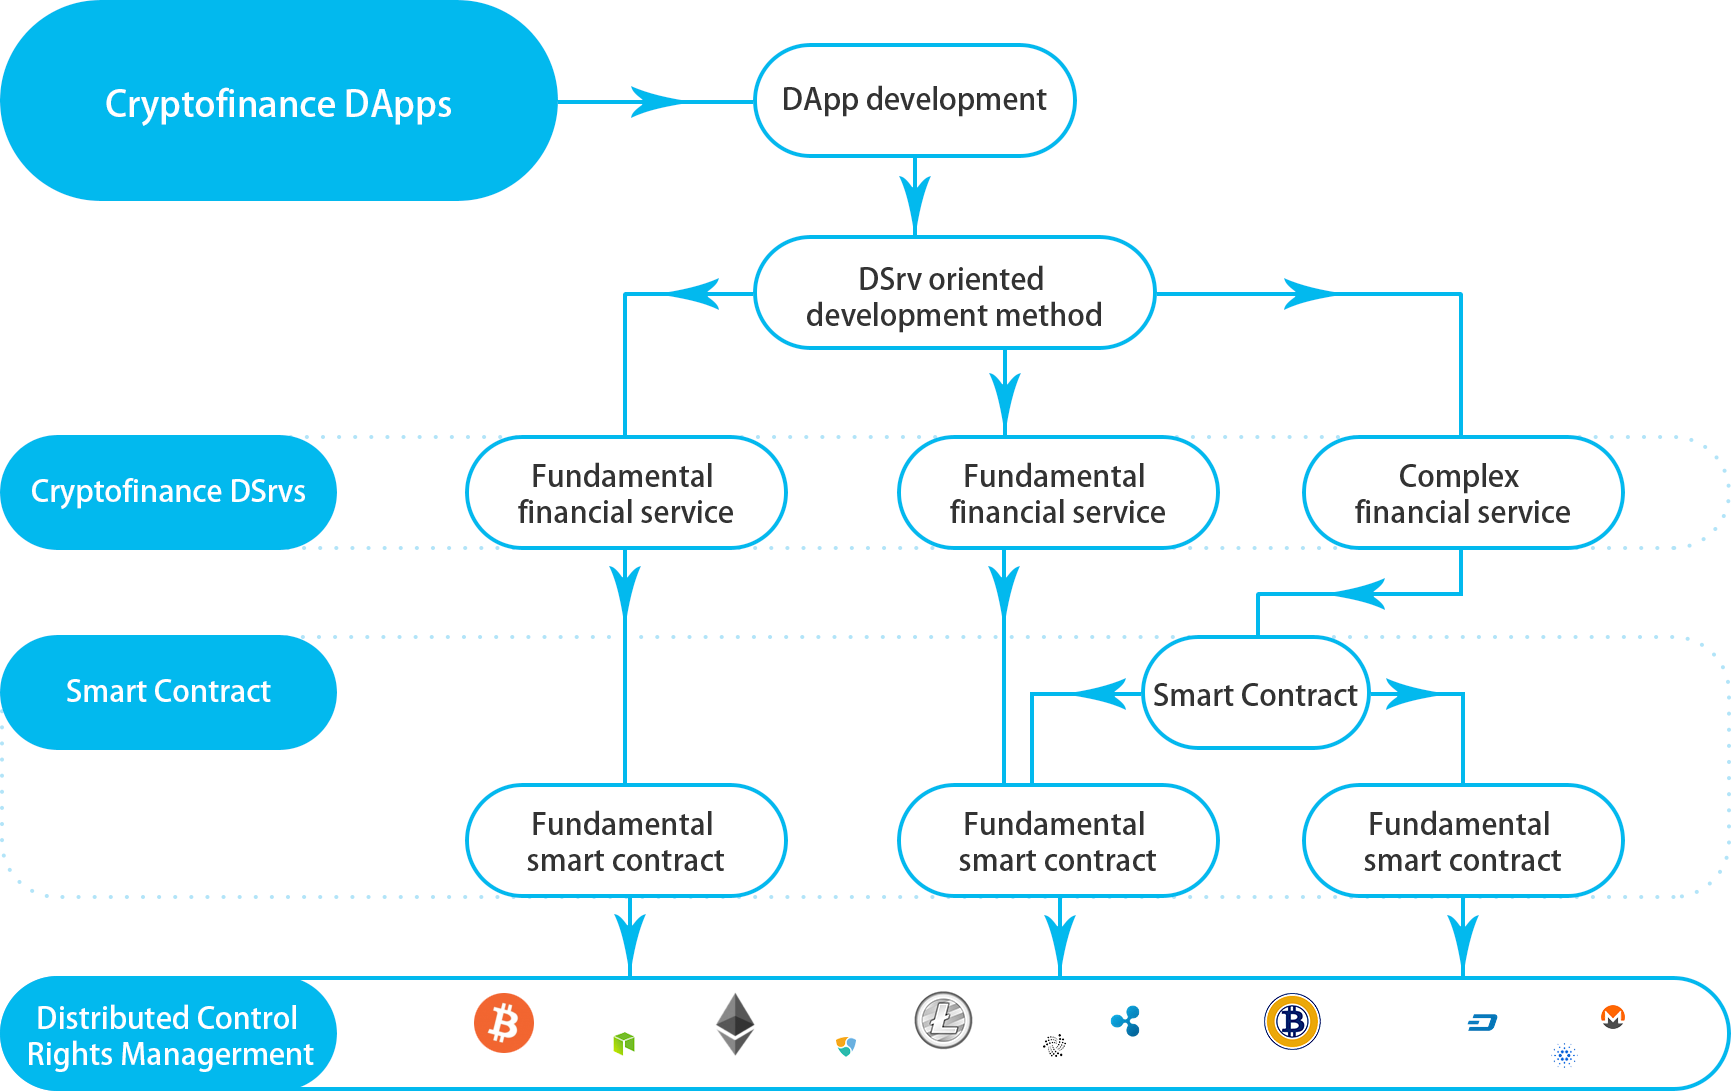
\includegraphics[width=5in]{pic/sccalling.png}
\caption{加密金融智能合约调用}\label{fig:1}
\end{figure}

FUSION将由基金会对基础的金融功能进行认定,从而形成智能合约库以供开发者调用。

(4)链外数据源接口

加密金融智能合约会在触发条件上使用链外数据。通常,此类数据获取是通过第三方提供的基于http或者socks的标准的API接口。例如,第三方接口调用函数会通过httpGet的方式获得目标url的地址,并返回一个json数据包。

这样接口方式同样适用于FUSION获取其他区块链上的信息,例如查询和确认其他链上某一笔交易是否得到所在区块确认的情况,也可以用于调入第三方的数据,例如Nasdaq当天的指数、欧冠的比赛结果、天气数据等等。

FUSION会由基金会对第三方接口进行认定和管理,并形成相应的第三方接口供智能合约调用。

(5)快速开发

项目初期,FUSION将提供一些典型应用的智能合约模板,供应用开发方参考和使用。但是,应用开发方在代码技能方面仍需具备一定的要求。

随着平台上基础功能和具有共性的金融基础应用越来越丰富和成熟,应用开发方可以通过预置条件调用这些智能合约以实现设想中的金融应用。为了进一步完善这样的开发环境,FUSION在之后的项目计划中包含可视化和模块化的应用开发工具、编译环境和应用测试环境的开发计划,从而极大地降低对来自金融交易领域的开发者的开发门槛,使他们可以聚焦于在FUSION上实现金融应用的创新。

(6)编程语言和虚拟机

在编程语言方面,初期FUSION将采用以太坊的Solidity语言,以实现智能合约的兼容和对现有智能合约的快速移植。后期,我们还将提供不同语言的编译器,从而实现对更多智能合约开发语言的支持。

我们将开发智能合约的沙箱运行机制,使用浏览器或编程编辑器就可以进行专门的防错检查和燃料费用优化。

在虚拟机方面,初期从兼容性角度出发将采用EVM的虚拟机,远期将考虑对于JVM进行裁剪和优化,实现JVM在FUSION中的移植和应用。这主要是考虑JVM是一个成熟而功能完善的虚拟机,有助于更好地实现更为复杂的金融应用并利用现在JVM上众多的开发资源。

\subsection{使用多条件触发实现复杂金融功能}

现有智能合约只能被动的等待一个交易的触发才能执行,这就造成了需要引入信任中介来决定谁有权利触发智能合约,在什么条件下触发智能合约的问题。FUSION平台上的智能合约通过代码约定多方之间的关系(不管是一个普通智能合约,还是嵌套智能合约),并使用多种触发条件自动触发的机制使智能合约可以在不需要人为触发的情况下相继运行,从而实现多方可以共同相信作为代码的智能合约,并完成各种复杂的金融功能。FUSION智能合约能够实现基于时间或者条件的触发,智能合约可以在整个运行过程中借出使用权并在不受任何干扰的情况下按照原来的约定进行执行,直到最后使用权与所有权返回给参与者。

这样的特性使智能合约能够实现各种金融功能。以借币参与ICO的应用场景为例,FUSION智能合约能够通过编程实现借币代投,并将代币、新币和利息原路返回的能力。以基金应用为例,在FUSION平台上的智能合约能够很容易实现基金的自动管理,投资人将各种代币使用权投入智能合约,投资各类加密数字资产,并通过条件触发产生管理费、分红和退出。以各种衍生品为例,在FUSION平台上可将保证金锁入智能合约,并通过外部数据源自动触发并追加保证金、平仓和结算等功能。
\section{分层混合共识机制}

\subsection{任务和共识的分层}

\subsubsection{分层混合的定义}

FUSION所采用的{\bfseries 分层混合共识机制(Hierarchic Hybrid Consensus Mechanism, HHCM)}是将区块生成的计算工作分层完成,并在不同分层中采用合适的共识机制。HHCM引入分组的概念以实现私钥生产、管理和并行计算。HHCM结合了PoW和PoS各自优势的情况下实现安全、效率、规模等多方面的均衡。

其中的{\bfseries 分层(Hierarchy)}体现在,交易打包生成区块的工作分成两个阶段,先后在两层之中完成。分层中的第一层为应用执行层,实现对于应用的执行,并将结果提交到第二层。第二层为区块创建层,将第一层提交上来结果打包形成区块记录到链上。

其中的{\bfseries 分组(Grouping)},分别体现在交易分组和节点虚拟分组上。在第一层——应用计算层中,由若干节点组成的虚拟分组完成当前所有交易中某一分组的计算,从而实现对当前所有交易的分组并行计算。此外,虚拟分组的形式增加了在每一轮中节点选取的随机性,增加了算法的安全性和扩展性,相关的论述将在后续进一步介绍。

所谓{\bfseries 混合的共识机制(Hybrid Consensus Mechanism)}体现在以下三个方面:
\begin{itemize}[itemindent=1em]
	\item 整个FUSION系统中参与区块打包的节点是基于PoS方式产生的。
	\item 在第一层的每个分组之中的共识也是采用PoS共识机制。
	\item 在第二层的区块生成过程中采用PoW的共识机制生成最终的区块。
\end{itemize}

下面介绍分层混合共识机制的结构和角色分工:

\begin{figure}[htbp]
\centering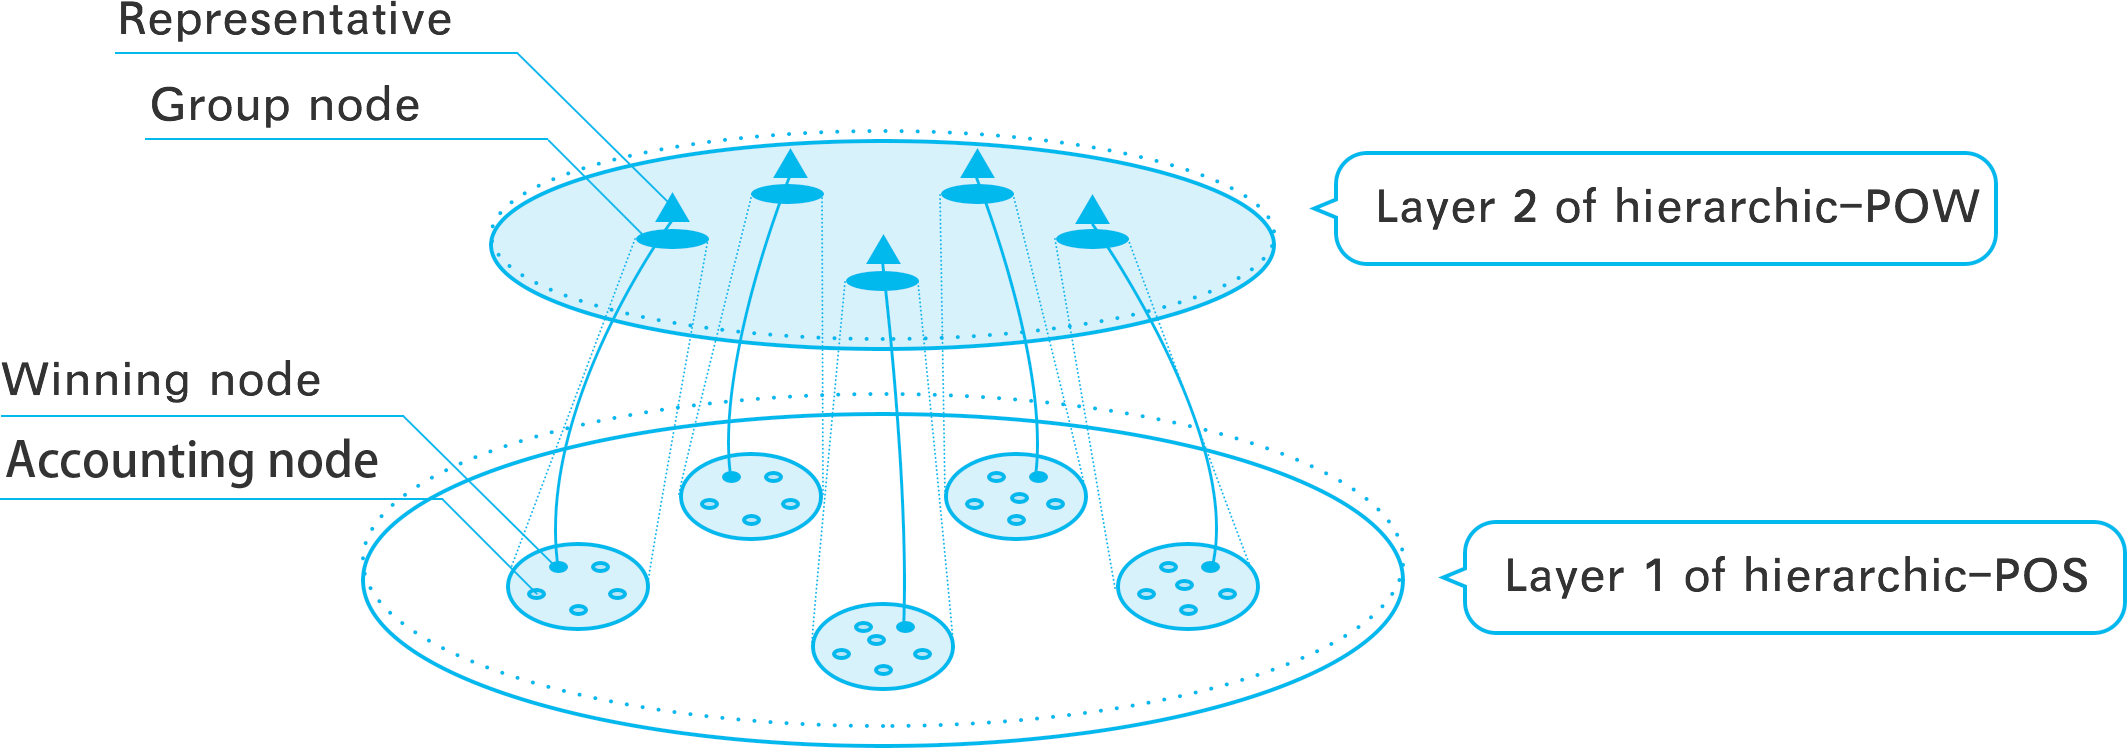
\includegraphics[width=5in]{pic/HHCA.png}
\caption{分层混合共识机制}\label{fig:1}
\end{figure}

以下对图中的角色加以阐述:

(1) 分层混合共识机制的第一层(Layer 1 of HHCM)

分层混合共识机制的第一层是由若干个物理记账节点组成的虚拟分组构成的。每个分组的节点将共同对分配给该组的所有交易中的一组进行打包处理,不同分组之间的工作是互不重叠的。

(2) 分层混合共识机制的第二层(Layer 2 of HHCM)

第二层中的节点是由第一层中某一个虚拟分组映射而来。在这一层中,将对第一层中所有组打包形成的交易包(Transaction Package)进行组合打包,最终形成新的区块。

(3) 记账节点(Bookkeeping node)

采用PoS的共识机制,从全网节点中选举产生的参与记账的物理节点。

胜出节点(Winning node),即这一组节点中竞争获得该组交易包(Transaction package)打包权的节点。

(4) 节点虚拟分组(Virtual group of nodes)

节点虚拟分组指第一层中由若干记账节点组成的分组。所谓虚拟体现在:

\begin{itemize}[itemindent=1em]
	\item 节点通过计算确定自己处于哪一个分组,而不是由谁指定分组及分组中的节点。
	\item 每一次组成虚拟分组的节点不同,并且任意记账节点并非每一次都处在同一个分组中。
\end{itemize}

这样的分组方式是一种动态的,不需要一个中心机制指定分组,所以称之为节点虚拟分组。

(5) 组节点(Group node)

组节点是指位于第二层中的,由第一层中的某一组节点映射而来的虚拟节点。组节点不是一个物理节点,只是将第一层节点进行虚拟分组,按照共识机制形成的胜出节点(Winning Node)。这个胜出节点作为该组节点的代表(Representative),与其他组节点的代表竞争完成区块的生成工作。

\subsubsection{分层混合的价值}

PoW是一种简单而有效的共识机制,但PoW也存在比较明显的问题,其中最引人关注的问题包括:
\begin{itemize}[itemindent=1em]
	\item 极高的能源消耗,并且随着系统规模的扩大而不断增加。
	\item 由于收益博弈导致算力的不断集中。这已经造成比特币在决策上的众多分歧而不断产生硬分叉。同时,算力集中也被认为是另一种形式上的中心化。
\end{itemize}

PoS是针对PoW的问题的改进了的共识机制。但随着系统的发展,PoS会带来资本集中化的趋势,造成越有钱越有权的情况。

FUSION的目标是实现通过各种数字资产之间的金融合约实现普惠的加密金融平台。它将是一个巨大规模的区块链金融应用平台。FUSION的共识机制必须在安全、高效的情况下,能够使系统性能适应应用规模、节点规模的不断扩大,需要同时控制能耗问题,并且避免产生各种形式上的集中。分层混合共识机制能够使系统安全、高效的运行,并且实现算力与权益的平衡,以及增强了系统的弹性。

\subsection{随机性与安全性}

共识算法的安全性有赖于每一次生成区块的节点的随机性问题。当恶意节点无法通过控制算力、控制权益或者攻击节点等各种手段确保获得连续区块生成的权利,就可以保障共识算法的安全性。

在关于随机性的理论上,FUSION在随机性的设计上与Algorand共识算法\citep{Jing2017}类似。大多数的PoS系统本质上也依赖于产生记账权归属的随机性来确保算法的有效性。Micali教授在Algorand中设计实现随机性的方式被称为“加密抽签”,即通过一种计算使选节点的产生有抽签的效果。FUSION这方面的随机性产生的方式与Algorand类似,也是通过一种计算来实现结果的随机性,从而确保每次分组的结果都具有不可预测性。FUSION这方面的随机性源于节点虚拟分组的实现,这点与Algorand算法在随机性的实现上不同。

下面是节点虚拟分组的产生过程中使用的方法:

\begin{itemize}[itemindent=1em]
\item 产生记账节点。FUSION上参与记账的节点是基于PoS产生的,此时持有更多权益和权益持有更长时间的节点具有更大的可能性成为记账节点。
\item 进行分组。FUSION将设定一个分组数量。节点可以通过上一个区块的hash值,以及另一个输入值,通过预先设定的一个函数计算产生一个结果。这里为了简化问题的说明,假设使用分组数量对这个结果取余,从而每个节点就可以知道自己所处的虚拟分组。分组过程是随机过程,与权益和算力无关。
\item 产生打包节点。在第二层中是以PoW的方式确定最终记账权的归属,与权益无关。
\end{itemize}

混合共识机制既使让记账权竞争者有动机拥有一定权益和算力,又不会使权益或者算力非常高的节点拥有过于集中的权力,同时保障了产生节点过程的随机性。当然,持有的权益最高、全网算力也最高的节点会具有更多的机会,但仍然难以确保频繁胜出。更重要的是,这样的节点已经与FUSION系统形成了巨大的利益共同体,没有理由去破坏自己的利益。

综上所述,虽然节点为了实现较大的记账机会,而花费大量的成本持有权益或者增加算力,但并不能确保胜出。同时,系统通过调整分组数量,将使得建立绝对算力优势需要无限趋近于全网算力,这将在算力与权益的平衡部分讨论。而没有持有大量权益或者绝对算力优势的节点,仍然有足够的机会获得记账权。这样更多的节点会更加趋于理性地对待在权益和算力上的投入,最终使大节点大都处于一个平均水平的状态。并且,随着网络节点数不断增加,这种均衡性并不会出现较大的变化,这个将在关于系统规模的伸缩性中进行讨论。

所以,HHCM将始终保持很高的随机性。

\subsection{算力与权益的平衡}

分层和分组的形式实现了高质量的随机性,也同时实现了算力与权益的平衡。

由于全网的记账节点是以PoS为基础从全网节点中产生的,这样可以在节点数量不断增加的情况下仍然能够保持一个合理有效的记账节点的数量。当每个分组产生胜出节点,由它们代表所在分组进入到第二层进行区块生成,这时按照PoW工作的节点数量等于系统约定的分组数量,这个值将始终可以有效地控制在一个可以接受的范围之内,由此采用PoW方式带来的资源消耗问题也是可控的。

通过这样的方式,FUSION在不同分层中采用不同的共识机制,是一种混合的共识机制。这种共识机制可以有效避免由于单独采用PoW和PoS所带来的突出问题,并且能够实现算力和权益之间的有效平衡,从而发挥两者的优势。同时,这也将真正吸引有志于参与FUSION的算力提供者和利益相关者。

\subsection{实现并行计算}

\subsubsection{并行计算}

分层混合机制带来的另一个好处是能够实现应用的并行处理。

并行处理体现在分层混合机制的第一层中。由于这一层构建了节点虚拟分组,同时也对同一个区块周期中所有的交易进行了分组,两者之间是一一对应的。在这样的情况下,每一个虚拟分组将对应处理所有交易中的一组交易,不同虚拟分组之间的交易是不重叠的。各个分组对各自交易计算的结果进行打包,成为在第二层共识过程中的输入,通过第二层对这些包进行再打包产生记账区块。由此,分层混合机制的结构通过分组实现了并行处理。

这样的交易并行处理在应用规模越来越大的情况下,具有越来越大的优势。只要通过调整与总交易规模相匹配的分组数量,系统就可以获得出色的并发性能。在设计的分层混合共识机制中,通过平衡算力和权益带来的优势,使得新加入的节点都有机会胜出获得区块打包的奖励,那么在应用丰富和交易量持续扩大的情况下,将自然形成吸引力,促使新的节点和算力不断的加入。

\subsubsection{规模的伸缩性}

采用分层混合共识机制,对FUSION在系统规模的扩容方面具有极大的价值。这也是当前区块链系统面临的重大挑战。

一方面,上面已经介绍了不论FUSION节点规模扩张到什么程度,即使达到百万节点的规模,通过动态调整分组数仍然能够把控最后参与到竞争记账权的节点数量在一个合适的范围内,从而推动整个系统高效、平稳的运作。

另一方面,在第一层应用计算过程中实现了以组为单位的并行计算,这使FUSION在面临金融交易规模不断扩张的情况下,可以通过增加更多的节点虚拟分组实现更好的并行处理能力。

因此,通过采用这样的共识机制,使得FUSION不论对于全网节点规模的扩张还是金融交易规模的扩张,都具有极好的伸缩性进行适应。

\subsubsection{应用分层的拓展}

第一层与第二层的工作是各有侧重的:第一层以完成应用执行为主要任务;第二层是对第一层的结果生成记账区块。这样的结构具有实现应用分层的先天优势,这能解决目前众多区块链系统节点存储数据规模过大的问题。

在FUSION中,对应用交易输入数据的存储和计算在第一层中完成,向第二层递交的是交易和交易结果。这些少量交易数据在第二层被打包成新区块。这样可以有效控制FUSION区块的大小在一个合理的范围内。合适的区块大小有众多的好处,比如有利于控制分布式网络中广播的效率,降低节点算力的要求,控制节点数据存储的规模,这些都有助于系统支撑大量的加密金融应用。

\subsection{分层混合机制的实现}

\subsubsection{分组的确定}

FUSION将为虚拟分组的建立设定一个计算公式,通过这个公式随机产生计算的结果并完成分组。随机性有助于确保整个系统不受恶意节点的控制。由于FUSION的所有功能和应用都对应到智能合约,因此在每一种智能合约中设定了自己对分组数量的值。

分组实现是由智能合约设定一个$X$,FUSION对分组确定的函数是$f(y,z)$。对于函数$f(y,z)$的输入条件$y$的取值是上一个区块的hash值(pre-Block hash),设为$\alpha $;对于条件$z$的输入是节点的公钥地址(Public Address),设为$\beta $。

则通过公式$$f(\alpha,\beta)\bmod \ X$$

每一个记账节点即可以确认自己所在的分组,这种分组的实现是完全去中心化的。

\subsubsection{区块的生成}

智能合约中的函数将它的交易定义成$X$组。节点可以通过上面的算法确定自己该领取哪一分组交易的计算任务。从而在这些节点之间就形成了相对于同一组交易而构成的虚拟分组。同一分组的节点按照PoS的方式确定哪个节点获得所在组的交易包(Transaction Package)的打包权。

每一个分组将诞生一个获得打包权的节点,也就是胜出节点(Winning Node)。由该节点作为所在分组的代表(Representative),进入到第二层,与其他$X-1$个代表(Representative)按照PoW的方式竞争该区块的打包权。

新的区块,将由对$X$个交易包的散列计算生成,新区块的打包者将是这$X$个代表(Representative)中的一个。

至此,完成分层混合共识机制下的区块生成。

显然,在节点实现虚拟分组的同时,智能合约也将交易进行了对应的分组,所以在分层共识的第一层中,各个组之间的工作任务是完全独立的,因而在第一层中实现了组与组之间应用处理的并发。

这样的设计,非常适合于FUSION对不同数字资产Lock-in的实现。甚至于Lock-in的智能合约不必等上个周期的Lock-in任务全部确认,而随时可以对新的Lock-in请求进行响应。由于每一笔Lock-in交易都要等到确认对象在原链上控制权转移的完成,这就造成了Lock-in请求在响应与最终完成写入区块之间是松耦合的关系,相当于分步完成。最终,在一个区块周期内,确认在原链完成Lock-in的交易,会被作为成功的交易打包进入这个周期的区块。这样FUSION就可以实现对于Lock-in这样高频次请求的快速响应,同样的Lock-out请求也可以按照这样的方式实现快速响应。

\subsubsection{随机性增强的探讨}

在分层混合共识机制的设计下,获得上一个区块打包权利的节点,在下一个区块打包的过程中,并不具有特别的优势。它可以通过自己生成的区块hash值,提前对自己在下一个区块周期中的分组有所了解,但是仅此而已。

对于另一种假设的探讨:假设被分配到$A$组的某个节点,去获取$B$组的交易进行打包。那么首先它将面临与$B$组节点的竞争,并不能保证该节点一定获得B组的交易包(Transaction Package)打包权成为胜出节点(Winning Node)。

即使该节点顺利成为了$B$组的胜出节点(Winning Node),在向智能合约提交$B$组打包结果的时候,该节点不具有打包$B$组交易的情况,会被智能合约通过分组公式检验出来,而被丢弃。因此,在这样的情况下,该节点只是做了一次100\%得不到任何奖励的无用功。同样的,一个恶意的节点也不能指望用这样的方式能够掌控连续的两个区块而形成双花的情况。

同时,分层混合共识机制仍然可以进一步增加其中的随机性。智能合约可以将$X$组中的一组设计为游击节点,而将所有的交易划分成$X-1$组。所谓游击节点,就是这些节点被赋予可以选择任意一组加入。

加入的方式就是游击节点可以任意选择交易分组中的一组数据进行计算,这样游击节点就加入到了该交易分组对应的节点虚拟分组中。同时,智能合约在收到交易包结果的时候,可以根据之前确定分组的公式进行判断,对于来自于游击节点的提交,则会被视为有效而正常接受。

在这个情况下进一步讨论随机性与安全的关系。假设全网中的节点都是善意和诚实的,那么游击节点的存在必然将进一步增加节点虚拟分组内节点组成的随机性,对最终获得打包权的结果产生更大的不确定性。

不确定性增加了恶意节点通过攻击节点获取区块打包权的努力,在即使获得上一个区块打包权,或者控制少数节点的优势会被随机性淹没,并不能确保它能够获得下一个区块的打包权。而攻击并掌控过多的节点,这个数量至少要大于等于分组的数量,但这已经是一个很大的数值,会引起整个系统注意。还有一种途径是对获得最后区块打包权的节点进行攻击,但是这也已经不能影响当前这个区块的结果,而下一个区块并不能保证依然有这个节点获得,这样的攻击是没有意义的。

接下来,我们讨论集中化对于FUSION系统安全性的影响。

如果存在一个有意控制FUSION的恶意方,希望通过获得足够多的游击节点数量,并且有意识地安排游击节点分别获取不同的分组交易数据来控制区块的生成。由于成为记账节点先要通过分组内的PoS,那么该恶意方首先需要为每个节点持有足够数量的权益,同时节点的数量要大于等于分组的数量,那么总共需要花费的数量将是两者的乘积。并且,每个节点需要确保在各个分组中以PoS的方式胜出,或者至少由它控制的胜出节点的算力总和在所有胜出节点算力的总和中达到51\%以上,才能保证在第二层PoW的过程中占有优势。则该恶意方需要为这些节点配置的权益将远远高于平均值,接近于最高值,并且还要为每一个节点增加足够多的算力,那么这个总量将会是一个无法接受的数字。同时,对于系统来说,对虚拟分组的数量增加一个数量级,并不会对系统的运作带来太大的压力,而对于该恶意方来说相应地新增足够数量的节点,将增加一笔很大的资金投入。在此情况下,它一定是FUSION中最大的利益持有者,用这种方式对FUSION发起攻击而使得所持有的FUSION权益清零,将是不现实的。

\section{项目计划}

\subsection{项目实施步骤}

\textbf{分布式控制权管理功能}

项目第一步是实现多代币分布式控制权管理功能,前端是一个能够存入和取出各种代币的钱包。钱包使用者将代币转入FUSION的地址,就实现了代币向FUSION平台的映射,感觉上与普通钱包没有任何不同。

由于这些代币是由分布式节点控制的,这里关键要解决的是私钥对节点不可见,节点有足够的激励保存私钥片段以及平台足够安全。

\textbf{多币种智能合约平台}

FUSION将为加密金融应用的开发提供一个基于多币种智能合约的创新平台的基础平台及相关外围设施。

\textbf{为各种中心化组织和外部数据源提供接口}

FUSION将为重要的中心化组织和外部数据源提供接口,以使更多的价值和数据源能够成为智能合约的编程对象。特别是身份数据,需要线下中心化组织的认证服务,而数据源要求稳定可靠。

\textbf{持续开发}

平台将不断在并行化计算、DSrv实现、共识机制等方面改进与升级,将平台发展为类似支付宝的高吞吐量的去中心化的版本。FUSION将不断培育应用市场,增加精品智能应用、代币种类和接口种类。FUSION将不断展开与中心化组织、数据源的合作,不断推进区块链接口的标准化运动,使越来越多的价值能够运行在平台上,实现普惠加密金融平台的愿景。

\subsection{社区运营计划}

\subsubsection{社区就是一切:新时代需要新办法}

FUSION加密金融平台是一条公共区块链,FUSION基金会作为项目的发起人,是为了一种很有前途的区块链生态而努力,而不是像传统企业项目运营那样为了公司盈利。FUSION平台作为一个普惠各种代币持有者的基础加密金融平台,不属于任何一个组织或个体,是属于整个区块链代币社区的平台。FUSION让代币的使用更加灵活,流通更加方便,更重要的是赋予了代币加密金融服务的功能。让所有的代币有更大的价值。事实上,价值互联网跨链生态是一个大事业,需要FUSION基金会发起,整个社区一起加入和参与,并通过不断的迭代产生越来越完善的区块链。这正是区块链项目的特点。区块链项目开始于一个重要的需求或待解决的问题,开发过程中需要由这些需求者和参与人不断的探索。与此同时,吸引社区中更多人参与,然后需求又向着更完善的方向发展,并进一步推动技术进步。所以,项目运营的思路必须一开始就是社区化的,社区运营关乎区块链的成败。

社区组成包括:
\begin{itemize}[itemindent=1em]
\item FUSION基金会和开发团队,是项目平台的发起者和推动者。
\item 对项目感兴趣的程序员。他们对项目或项目技术感兴趣,可以加入基金会开发团队,或者作为第三方独立开发优化FUSION。
\item FUSION参与节点。通过记账获取收益,并维护FUSION的运营。
\item FUSION平台的使用者,通过使用FUSION平台获取加密金融服务。
\item FUSION平台上的加密金融服务提供方,比如支付平台,中心化或非中心化交易所,借贷平台等金融服务提供方。
\item Fusion代币投资者。包括私募机构、早期投资者、后期投资者和潜在投资者。
\item 其它相关者。包括媒体、政府等等。
\end{itemize}

以上人士或组织都对FUSION未来发展起着重要作用。社区运营的目的就是尽量调动最多的力量,以最有效的方式组织起来,让FUSION能够不断迭代,形成影响力,并服务于更大的社区。

社区的成长,其实与核心社区和外围社区都有关,两者也是相辅相成的。核心社区是内核,但关键社区的形成需要外围社区不断的吸引人进入,因为核心社区的人来源于外部社区,但外围社区也需要核心社区的资源的支撑。我们发现比特币、以太坊等项目的成长都遵循了这一规律。我们将核心社区定位于初期创始者、区块链技术社区、区块链投资社区,外围资源则是其它对项目感兴趣的投资者、使用者、开发者、媒体等等。

\subsubsection{项目推广方法}

本项目将社区运营分为两方面:核心社区和外围社区,前者主要采用线下方式,后者主要采用线上模式 。在核心社区运营方面的计划是:

\begin{itemize}[itemindent=1em]
\item FUSION基金会团队:我们将给团队一定的代币奖励,一是补偿前期投入的资源,二是让其能够成为权益关系人,期望未来继续投资持续参与FUSION发展。
\item 区块链技术社区:技术是区块链发展的核心和难点。我们将利用创始团队的技术力量和社交资源, 以线上和线下两种方式,发掘、培育一批技术顶尖的人才,以促进技术社区的状大。
\item 区块链投资社区:以区块链技术社区为依托,通过投资人见面会的形式,我们即能向私募等投资社区的人士普及区块链知识,也能增进双方的合作机会。
\end{itemize}

\subsubsection{区块链技术促进活动}

价值互联网目前在可用性方面还存在瓶颈,并且需要未来作出持续的努力不断促进其可用性。FUSION项目与价值互联网的可用性息息相关,我们将发起“区块链技术促进运动”,为区块链技术在可用性方面的进步贡献力量。这将是基金会一项长期的工作。

该运动线下将以技术沙龙、训练营、专题研讨的形式不断聚集人才和技术资料。我们将推进线下参与人员提供内容,以各种网站和各种媒体的形式推广内容。并通过不定期的办班的方式来吸引传统互联网的人员和其它技术人员以扩大技术社区的后备力量。

区块链技术促进运动将团结一切可以团结的力量,包括高校、研究所、企业、机构、政府、联盟等建立合作关系,并聚集资源合力推动区块链技术的进步。

\subsubsection{区块链接口标准化运动}

价值互联网在互通性和可扩展性方面还存在瓶颈,并且需要多方参与完善。FUSION项目与价值互联网在这两方面的进步息息相关。我们将通过发起“区块链接口标准化运动”,为价值互联网在互通性和可扩展性方面不断进步贡献力量。这将是基金会一项长期的工作。

特别要注意的是,这场运动不仅提倡区块链之间的通过接口的标准化,也同时提倡与其它重要组织接口的标准化,以及与外部数据源接口的标准化。

\subsection{FUSION发展蓝图}

\subsubsection{任务及时间节点}

FUSION项目从2017年开始启动,已经完成概念验证,接下来的任务和时间节点如下(时间轴图见图\ref{fig:timeline})。

% \begin{itemize}
% \item 2017年下半年:(1)区块链发展现状的经济学理论分析和问题提出;(2)项目内容和意义讨论;(3)完成概念验证和项目启动;(4)核心团队组建;(5)平台架构设计和技术论证;(5)完成白皮书;(6)启动私募和项目顾问交流。
% \item 2018年一季度:(1)完成合规化工作,启动基金会工作,项目全面展开运营;(2)完成核心协议的开发,完成实验代码的编写,并开始进行多节点实验环境下的持续测试;(3)启动外围社区运营,并完成ICO工作;(4)启动投资社区、技术社区和高校等的核心社区运营工作,协力推进研发工作;(5)完善核心团队建设。
% \item 2018年二季度:(1)上线测主链;(2)展开密集的跨链合作,完成100亿美元的分布式控制服务;(3)继续推进核心社区发展,成立多个研究课题,大力推进研究工作;(4)完成智能合约浏览器和核心钱包的开发;(5)推进外围社区,展开密集的宣传推广工作;(6)完善团队建设。
% \item 2018年三季度:(1)完善前端钱包工具,完成1000亿美元的分布式控制服务;(2)展开外围社区的运营工作,完善智能合约开发工具,完成超过10亿美元加密金融应用;(3)不断完善核心代码的效率和安全性;(4)继续推进核心社区并协助他们参与进行创新性的加密金融功能实验开发。
% \item 2018年四季度:(1)继续推进核心代码的改进和完善;(2)继续推进核心社区及研究工作;(3)推进链下中心化组织的接口标准化工作;(4)推进链下数据源上链工作,特别是身份信息上链工作;(5)完成具有重要的中心化组织与区块链的接口工作;(6)继续完成生态系统内各种配套工具的开发。
% \item 2019年及之后,根据2017年及2018年的运营情况,进一步迭代产品,不断推进普惠加密金融平台的建设,使之成为价值互联网时代帮助人们提高金融效率最重要的发明之一。
% \end{itemize}

\begin{figure}[htbp]
\centering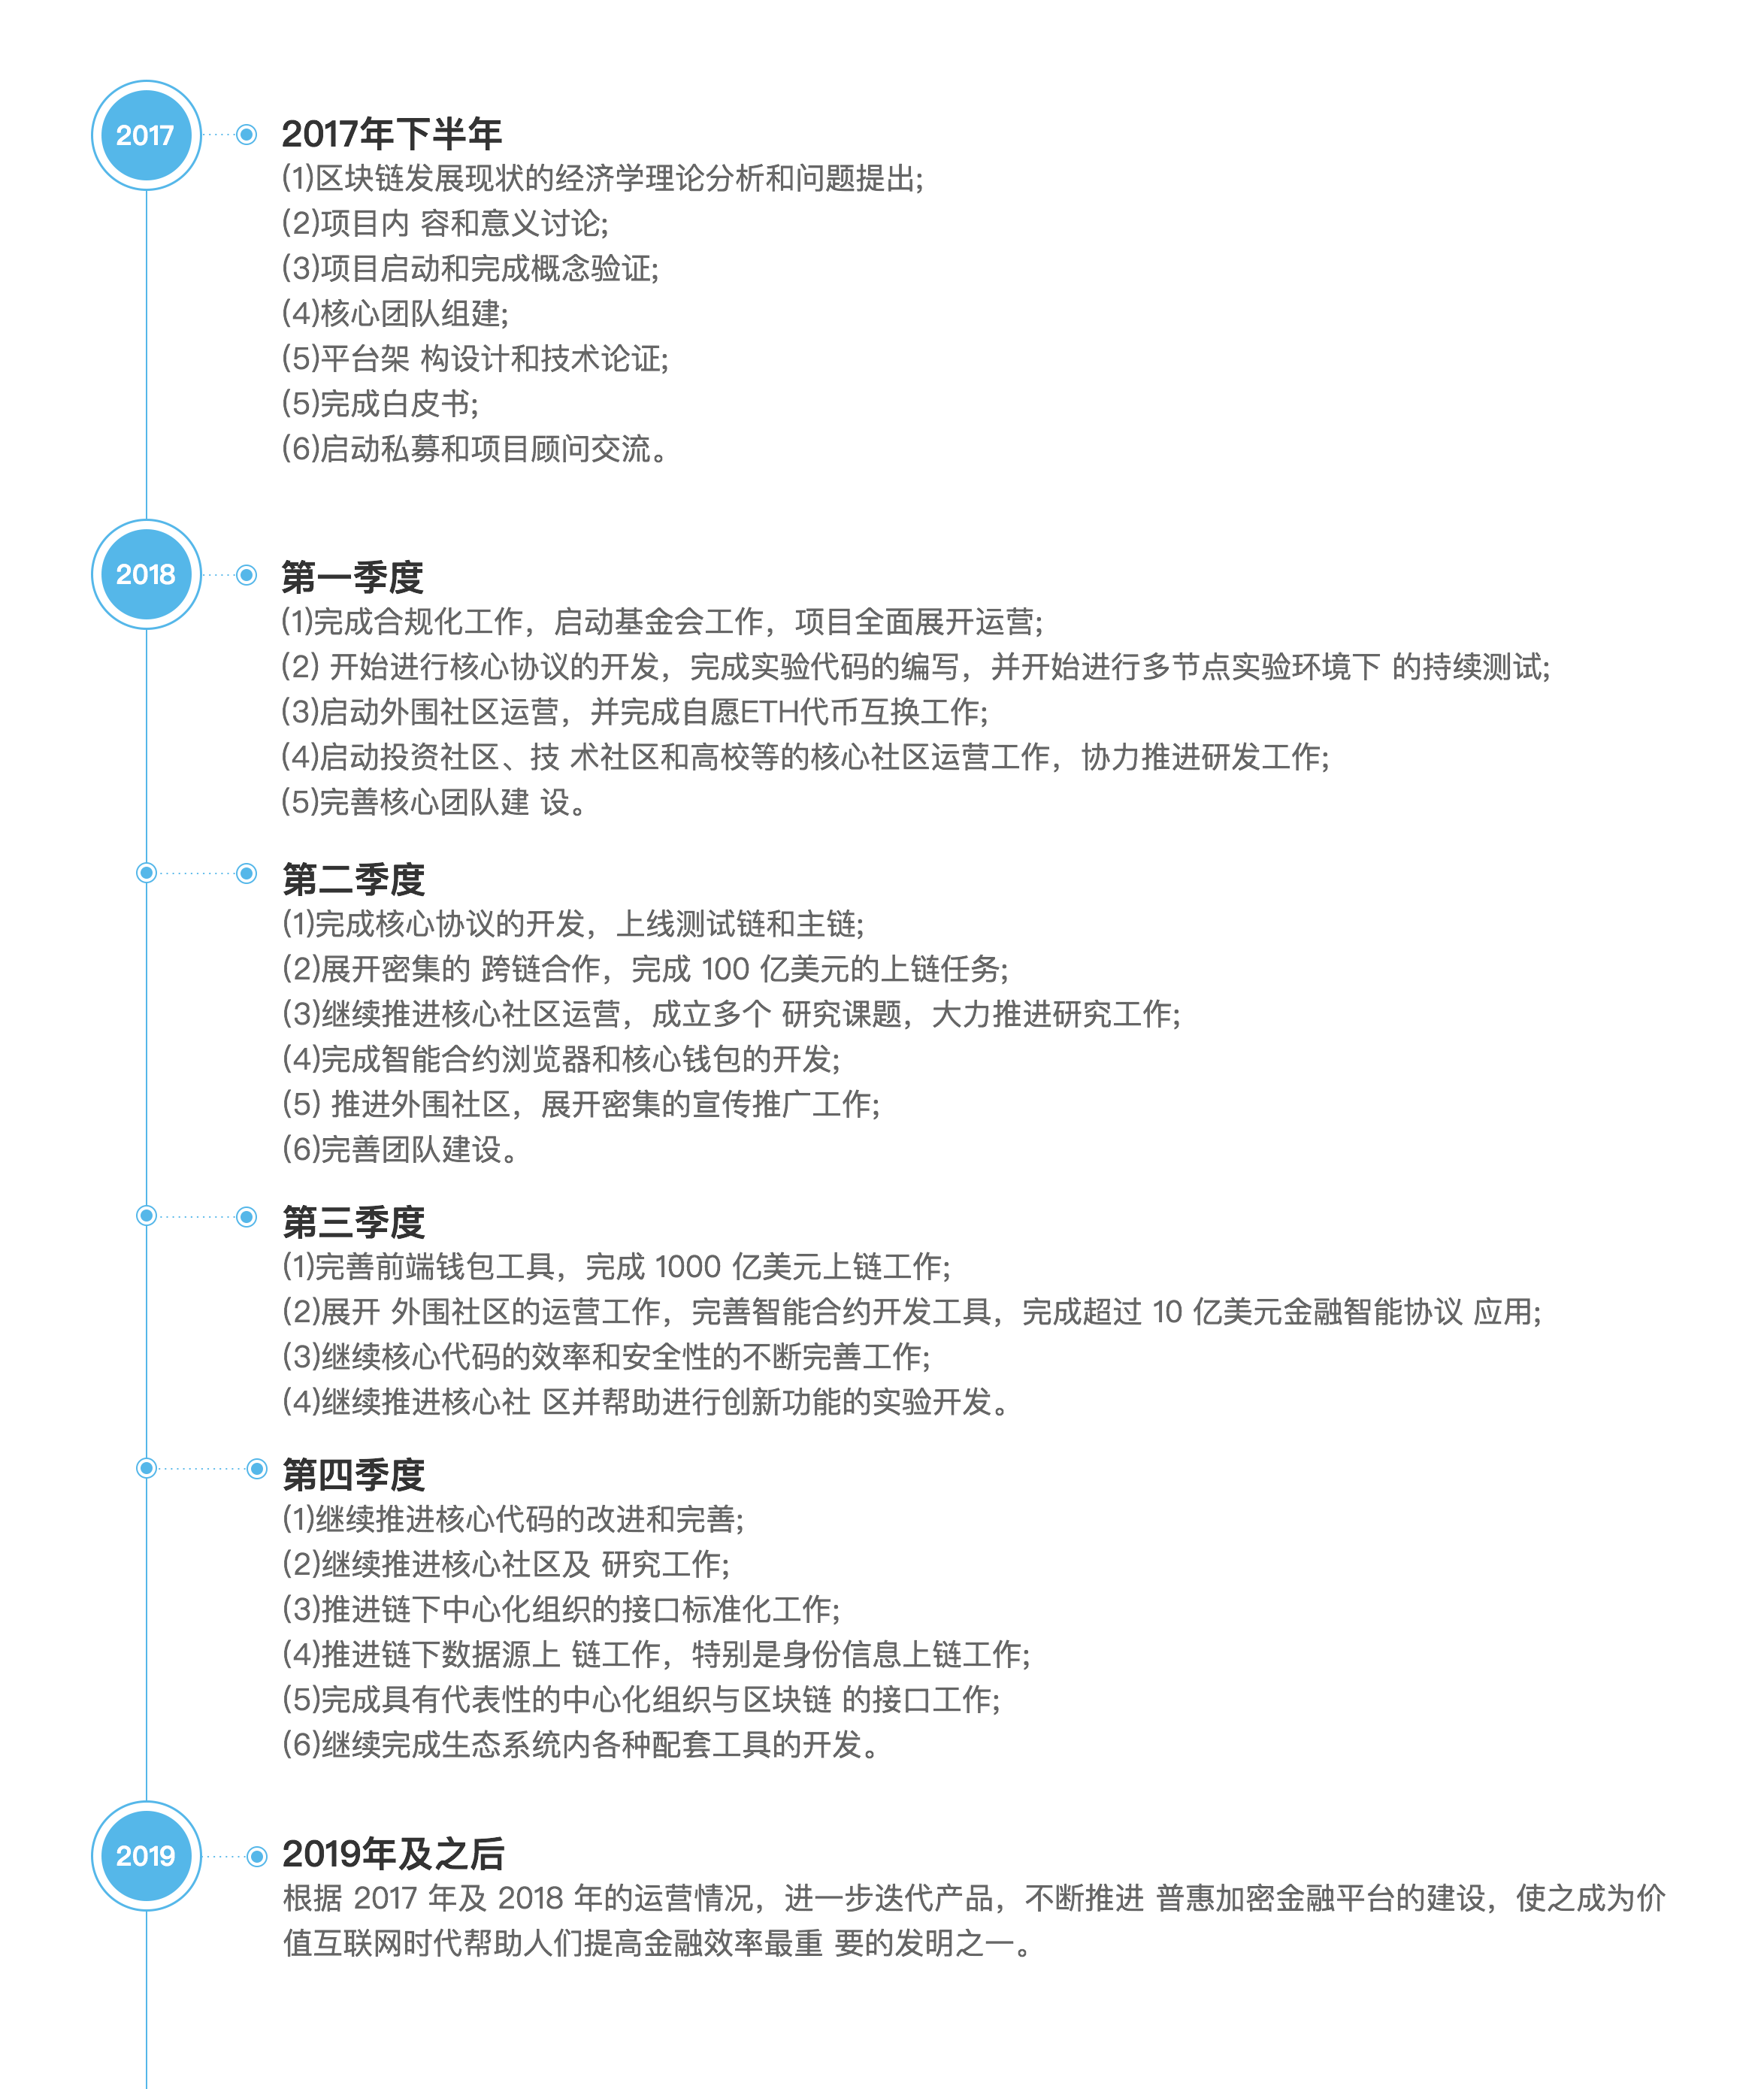
\includegraphics[width=6.6in]{pic_cn/timeline.png}
\caption{任务及时间节点}\label{fig:timeline}
\end{figure}

\subsubsection{代币设计与分布}

代币是公有链生态系统不可缺少的组成部分。它像是一个机械装置的润滑剂,又像生命系统的血液,更是公有链经济系统的激励机制。正是以代币为基础的共识机制把社区成员聚集在一起,实现区块链生态系统良性循环。对于项目初创者,代币是对他们付出的必要的补偿和未来继续参与的动力;对于使用者,代币就是通行证;对于投资者,代币是通向未来的门票;对于开发者,代币让他们成为股东;对于记帐节点,代币更是他们辛勤付出的补偿。所有持有代币的人,他们可以是上述多重身份,他们与公有链项目息息相关,成为使用者、宣传者、开发者、投资者,与项目生态一起成长,成就普惠加密金融平台及应用的伟大事业。

为了实现普惠加密金融平台的愿景,FUSION项目设计了Fusion(FSN)代币,并且设计了Fusion分布结构,以使项目可持续发展。代币在设计上主要考虑五个方面:

\begin{enumerate}
\item 数量。代币供应数量总共8192万个。8192是2的13次方。这个数量能够使代币上线时有一个合理的价格,并在此基础上稳步成长。
\item 代币发行机制。代币供应应该有个上限,实现非通胀的理念。这使越早参与者越有利,也使系统稳定性不断增强。
\item 代币分布。代币在分布上必须有很好的平衡,实现非中心的理念。FUSION团队需要在跨链、跨组织和跨数据源上付出巨大的努力,我们分配10\%给团队。另外,因为FUSION记帐节点任务比较重,可以占近三分之一。而剩余的将用于生态建设。
\item 生态建设。超过半数的代币将用于基金会,促进项目不断成长,特别是跨链、跨组织和跨数据源方面。项目也需要有一套货币互换的机制,让更多价值能够到链上表示,并且激励开发新的智能合约应用。
\item 矿工和燃料。各种价值将以分布式节点控制的方式进入到FUSION,需要大量的分布式节点控制代币,节点越多安全性越高。并且在链上运行的价值越大,越需要更多的节点。要维持节点数量和算力,就需要给矿工记帐奖励和服务费。

\end{enumerate}

代币的分布如下(饼图见图\ref{fig:tokenratio}):

% \begin{enumerate}
% \item 团队激励:819.2万(10\%)分配给核心团队所有,分阶段分配给团队,以激励吸引更多精英的加入;
% \item 天使投资:819.2万(10\%)分配给天使支持资金,支持项目最早期的启动与开发;
% \item 代币互换:819.2万(10\%)用于基金会合作发展,与区块链社区与中心化组织的战略合作;
% \item 定向ETH募集:819.2万(10\%)分配给定向分配愿意参加ETH换FSN的参与者,所获得代币用于基金会项目开发团队运营;
% \item 自愿ETH互换:2048万(25\%)分配给向自愿参加ETH换FSN的参与者,募得代币将用于基金会,区块链应用生态发展;
% \item 保留用途:409.6万(5\%)将作为临时的储备,由基金会决定其未来用途;
% \item 工作量证明和权益证明:2457.6万(30\%)将用于工作量证明和权益证明共识机制激励。
% \end{enumerate}

% 团队激励:819.2万(10%)分配给核心团队所有,分阶段分配给团队,以激励吸引更多精英的加入;
% 天使投资:819.2万(10%)分配给天使支持资金,支持项目最早期的启动与开发;
% 代币互换:819.2万(10%)用于基金会通过代币互换发展合作关系,包括与其它区块链社区或中心化组织的战略合作;
% 定向ETH募集:819.2万(10%)分配给定向分配愿意参加ETH换FSN的参与者,所获得代币用于基金会项目开发团队运营;
% 自愿ETH互换:2048万(25%)分配给向自愿参加ETH换FSN的参与者,募得代币将用于基金会,区块链应用生态发展;
% 保留用途:409.6万(5%)将作为临时的储备,由基金会决定其未来用途;
% 工作量证明和权益证明:2457.6万(30%)将用于工作量证明和权益证明共识机制激励。



\begin{figure}[htbp]
\centering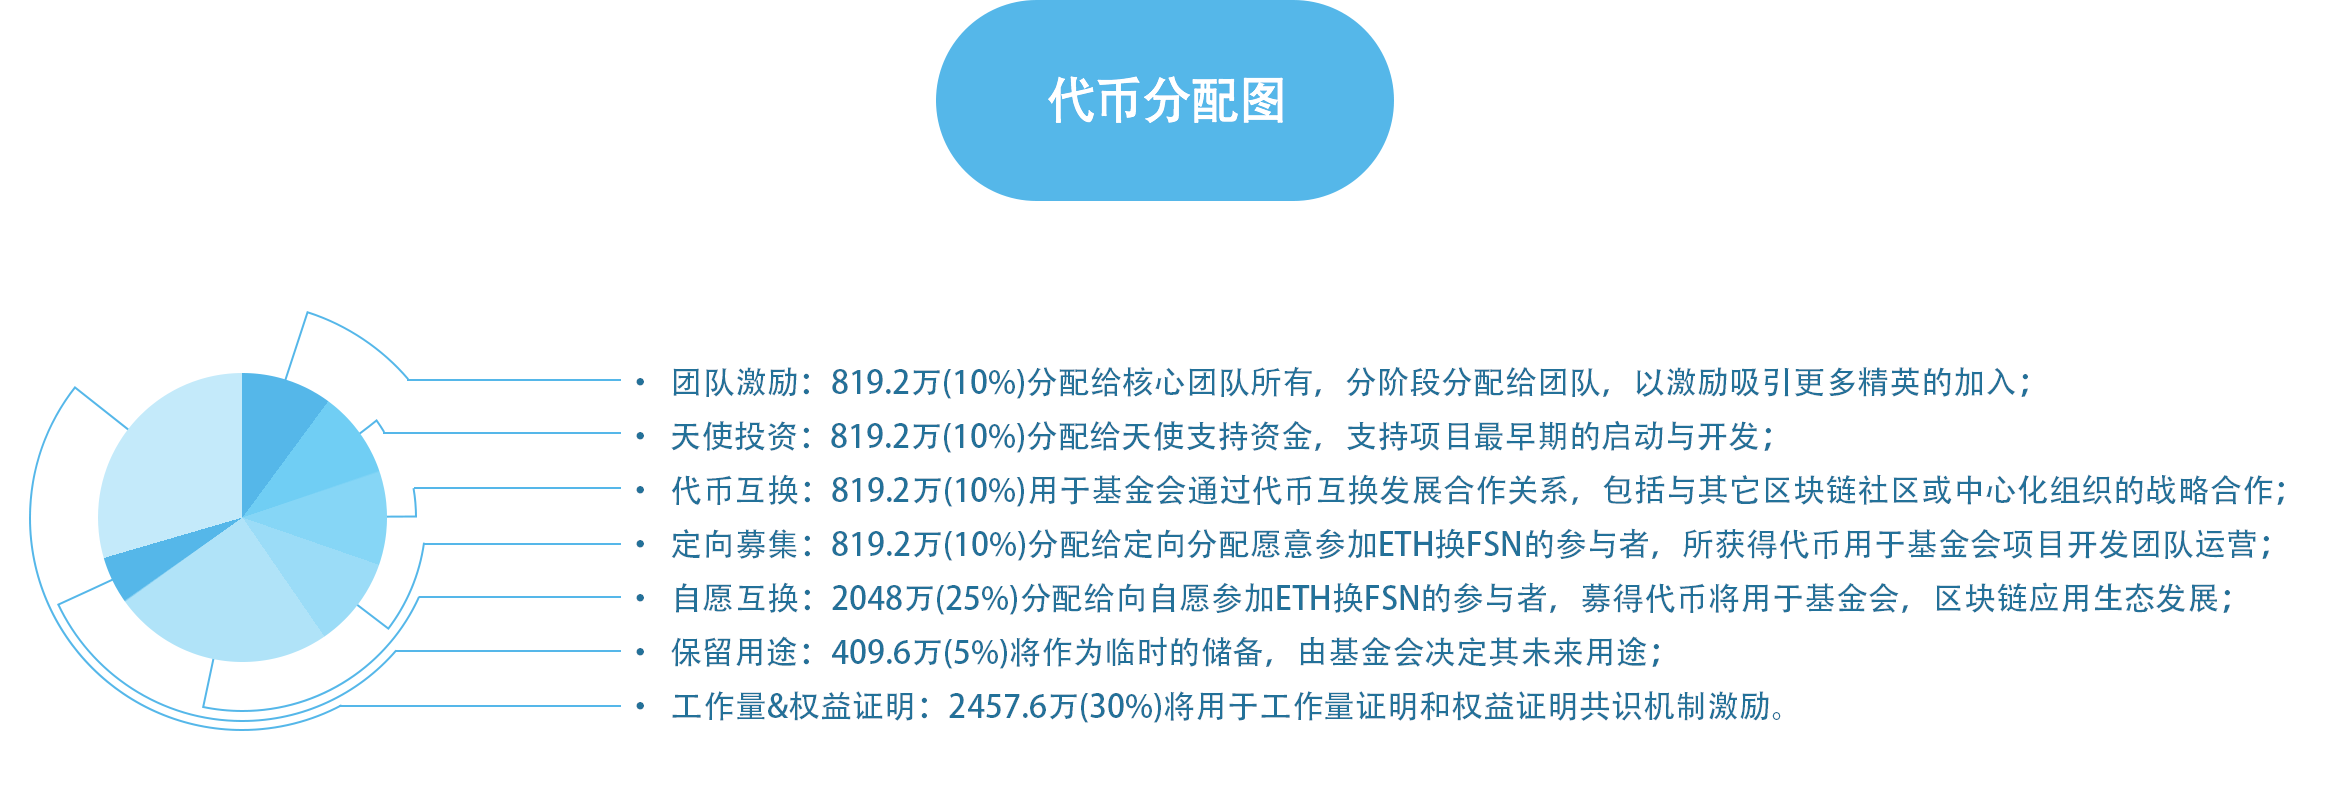
\includegraphics[width=6in]{pic_cn/tokenratio.png}
\caption{代币分布}\label{fig:tokenratio}
\end{figure}

%\renewcommand{\appendixname}{附录~\Alph{section}}

\appendix
\clearpage
\renewcommand\refname{参考文献}
\bibliographystyle{fusion}
\bibliography{fusion}
\clearpage
%\renewcommand\appendixname{附录}

%\theendnotes
\end{document}

%%% Local Variables:
%%% mode: latex
%%% TeX-master: t
%%% End:
